\documentclass[a4paper]{article}
\usepackage[hmargin=1in, vmargin=1in]{geometry}
\usepackage{makeidx}
\usepackage{fancyhdr}
\pagestyle{fancy}
\usepackage[pdftex]{graphicx}
\usepackage{amsmath}
\usepackage{amssymb}
\usepackage{listings}
%\makeindex
\begin{document}
\begin{center}
\title{Three dimensional coordinates into two dimensional coordinates transformation}\\
\author{Edward Gerhold}
\city{Berlin, Germany}
\date{\today}
\maketitle


Version 0.3.4-unstable-parts\\

\textbf{Remark. This is a development version. And has chaotic parts} This file contains typos, unwanted logical mistakes and miscounts, and a maybe accidental letters, which came from a suddenly appearing double cursor in the editor.\\
\\
\\
The current version is very informal since the last versions compared with very formal. That text is subject to be deleted asap.\\
}\\


\end{center} 


\tableofcontents\\

\section{Introduction}

On a piece of paper you see three coordinate axes pointing into three
directions in space. In reality these vectors are two dimensional. Because
they point into three directions on the paper, and not into the real space.\\

\begin{figure}[ht]
\label{ijksystem}
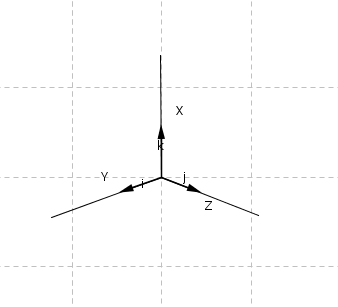
\includegraphics[scale=2]{ijksystem.png}\\
\caption{Picture of a right handed 3-D coordinate system with ijk-basis-vectors on the axes pointing
into three dimensions. See \cite{Corral1} for introduction.}
\end{figure}

In this document we will design a $\mathbb{R}^{2\times{3}}$ basis for the coordinate transformation. 
A basis is multiplied with the values of the coordinates to move for each component 
a piece, to end the move on the correct new point.
In the case of cosines and sines, we move left and right and up and down, to 
tell you directly, what happens, when we multiply the coordinates with the matrix.\\

\textbf{What we will do in the document}

\begin{enumerate}
\item Choose angles for our coordinate axes around the unit circle to lay out three axes.
\item Write down the basis vectors for each coordinate axis
\item Assemble a matrix with the vector basis for a point by point transformation.
\item Read the example source code for a computer function, which is exactly two lines long. One for the new $x$ and one for the new $y$.
\item Read other versions of the transformation, with functions, for example.
\item Derive the generic case of transforming coordinate systems down to the plane.
\end{enumerate}

\section{Designing a $\mathbb{R}^{2\times{3}}$ coordinate system for our transformation from $\mathbb{R}^{3}$ to $\mathbb{R}^{2}$}

\subsection{The $_{n}$ index for $_x,_y,_z$ with $_x=1$, $_y=2$ and $_z=3$}
\index{index}

The index $_{n}$ in $r_{n}$, $\varphi_{n}$, $\vec{e}_{n}$ is the index for $_x$,$_y$,$_z$. For example $\varphi_{n}$  stands $\varphi_x, \varphi_y, \varphi_z$. $r_{n}$ stands for $r_x$, $r_y$ and $r_z$. $\vec{e}_{n}$ is for $\vec{e}_x$, $\vec{e}_y$, $\vec{e}_z$ It is possible, that in the formulas $x,y,z$ and $1,2,3$ may be used interchangeably. For example, when summing up the products of the coordinate components with the basis components, this happens. The formula is $\sum_{i=1}^{3}\vec{x}_{i}\vec{e}_{i}$, which is a sum of $x,y,z$ and the $\cos \varphi_{n}$ terms in the first components of $\vec{e}_{n}$ for $x'$ and a sum of $x,y,z$ and the $\sin \varphi_{n}$ terms in the seconds components of $\vec{e}_{n}$ for $y'$.

\subsection{$\varphi_{n}$ the angles for the coordinate axes}

Why do we need angles? May be the first question. My answer is, we will arrange the basis vectors,
easily around a circle, by their angle. Since they are two dimensionsal. The circle is available in two dimensions.
With the arrangement around a circle, we get the right numbers, same lengths, instead of guessing wild numbers.\\

First draw three axes of a 3-D coordinate system on a piece of paper. Draw the horizontal x-Axis through the origin of the drawn coordinate system. You could directly add the y-axis, to see a 2-D coordinate system carrying your two dimensional 3-D system. A system with three vectors pointing into three directions, originating in the origin of the real R^2 space.\\

\begin{figure}[ht]

\includegraphics{handsystems.png}
\caption{A left-handed and a right handed coordinate system. They just have different angles in our 2-D projection.}
\end{figure}

Each of the three vectors has an angle, counted from the horizontal positive x-axis, going counterclockwise around the origin. The
angle between the axes themselves isn´t what we want. We want the angle beginning on the real 2-D x-axis, to feed the cos and sin functions with, when calculating the real numbers of each basis vector.\\

In this document, i will call the angles $\angle \varphi_{n}$ or just $\varphi_{n}$. If they are measured in degrees or radians depends
on the cosine and sine functions you use. And on how you would like to read your own definition.

Let $\varphi_{n}$ be the set of axis angles, one for each axis. I put them into a set in this document to simplify the access by
using the index $_{n}$ together with $_x, _y, _z$ or $1,2,3$. $\varphi_x$ or $\varphi_1$ is the angle of the x-axis. $\varphi_y$ or $\varphi_2$ is the angle of the x-axis and $\varphi_z$ or $\varphi_3$ is the angle of the x-axis. 


\begin{displaymath}
\varphi_{n} := \{\varphi_x, \varphi_y, \varphi_z\} = \{ \varphi_1, \varphi_2, \varphi_3 \}
\end{displaymath}

We will need the three angles for the axes shortly. So don´t forget it over the next lines.


\subsubsection{Degrees or radians?}

Depending on the cosine and sine functions and the input value for the angles, you may have to convert the degrees to radians, or
the other way round, the radians to degrees. For example, the JavaScript Math.cos and Math.sin functions take the values in radians.\\

\begin{example}
\textbf{example}
The function rad converts degrees to radians, it´s useful for computer functions taking radians.
\begin{displaymath}
\text{rad}(\phi) := \frac{\pi}{180} \times \phi, \phi \in \mathbb{R}
\end{displaymath}


Here is an example of three angles. The three axes have an angle of 120 degrees between each. But since we start counting counterclockwise and from the real horizontal axis of the plane, the angles are 210, 330, 90 in degrees, respectivly. And
because of the cosine and sine functions taking radians, we convert the values to radians.
 
\begin{displaymath}
\varphi_x = \text{rad(210)}, \varphi_y = \text{rad(330)}, \varphi_z = \text{rad(90)}
\end{displaymath}

\begin{displaymath}
\varphi_x &= \frac{\pi}{180} \times 210 &= \frac{7\pi}{6},  
\varphi_y &= \frac{\pi}{180} \times 330 &= \frac{11\pi}{6}, 
\varphi_z &= \frac{\pi}{180} \times 90 &= \frac{\pi}{2} 
\end{displaymath}
\end{example}

\textbf{example}
The function deg converts the other way round and from radians to degrees. You multiply your value with the reciprocal of PI/180, namely 180/PI and get the other way round.
\begin{displaymath}
\text{deg}(\phi) := \frac{180}{\pi} \times \phi, \phi \in \mathbb{R}
\end{displaymath}

\textbf{example}
The first example was for the righthand coordinate system. Here are the angles for a lefthand system.
\begin{displaymath}
\varphi_x &= \frac{\pi}{180} \times 0 &= 0,  
\varphi_y &= \frac{\pi}{180} \times 90 &= \frac{\pi}{2}, 
\varphi_z &= \frac{\pi}{180} \times 45 &= \frac{\pi}{4} 
\end{displaymath}


If you would like to get hands on angles, cosines, sines, or need a refresher, \cite{Corral2} is a good choice. And as well \cite{Corral1} and \cite{Strang2} teach unit circles, polar coordinates, sines, cosines and wonderful mathematics.

\subsection{$r_{n}$ is the length of the unit on each axis}

Before i show you the three vectors, and how to use them, we have to clear another piece of information belonging to each
basis vector. In this document it is called $r_{n}$. The r is from radius. And it stands for the length of the basis vector.
The length of the basis vector defines, how far a point in this direction will go by one unit.
\begin{displaymath}
r_{n} := \{ r_{x}, r_{y}, r_{z} \} = \{ r_{1}, r_{2}, r_{3} \}
\end{displaymath}

The $r$ originates from radius from the unit circle and from the parametrization of (x,y) via cosine and sine. 
In polar coordinates the cosine and sine are multiplied with r. Also to change the length of the hypotenuse, 
the vector $\vec{r}$, which is the third side to a triangle by cosine, sine and r. 
If r is left away, the length of the basis vector is 1. Or in other words, the distance $d((0,0),(x,y))$ from the origin to $(x,y)=($$r \cos \varphi$$, $$r \sin \varphi$$)$ is $1$, if $r=1$ or if r is left away completely.\\

Pay attention to this point now, to keep the affine transformation, especially under rotation, correct. You should give all three
axes the same r-value. I will define them in this document as $r_{n}$ with one $r_x, r_y$ and $r_z$ for each coordinate axis,
to keep it complete. But if you would like to change the units on your objects, i have to recommend, that you apply a local
3x3 basis with the disjoint unit lengths. This will keep the rotation correct. In the other case, the object would suddenly
stretch the head, if you rotate it to the side, where the unit for example is longer.\\

So for the coordinate system, the best setting is $r_x = r_y = r_z$. Keeping them equal, you can rotate it realistic. But you
don´t need to keep the unit length of 1 for the vector. Elonginating the units on the axes make zooming transformations very
easy.\\

\subsubsection{Taking the norm of $\vec{e}_n$ to obtain $r_n$}

If you have some existing basis and you would like to figure out, how long r is, you can go the other way round and take the
norm of the vector. Taking the norm means to measure the length of the vector. This is done with the euclidean norm, or the
2-norm for regular purposes.\\

$r_{n} = \sqrt{\vec{e}_{n}\cdot\vec{e}_{n}}$ = $\sqrt{(\vec{e}_{n},\vec{e}_{n})}$ = $\left(\Sigma_{i=1}^{2} \vec{e}_{i}^2\right)^{\frac{1}{2}}$ = $\|\vec{e}_{n}\|$\\itt

With this formula you can not only measure the length of the basis vectors, but any vector in the $\mathbb{R}^{3}$ and the $\mathbb{R}^{2}$ space. 
More advanced measurements include the p-Norm, which is $\sqrt[p]{\sum_{i=1}^{n}|\vec{x}_{i}|^{p}} 1 \leq p \leq \infty$ and $\sup_{i=1..n} |\vec{x}_{i}|$ for $p=\infty}$ and the max-Norm $\|\vec{x}\|_{\infty}$= $\sup_{} \{|\vec{x}_{i}| \}$. There are matrix norms like $\|A\| = \max_{i=1..m} \sum_{j=1}^{n}A_{ij}$, which for example yields the largest row of a m by n matrix. Norms are used everywhere ing mathematics for measuring the lenghts or getting the absolut values of the vectors and matrices. And the distance function $d(\vec{x},\vec{y}) = \|\vec{x}-\vec{y}\|$ is used to measure the distance between to points or two vector tips. A vector space V with a distance function $d(x,y)=\|x-y\|$. 
  is called a metric space $(V,d)$. And a complete metric space with a norm, written $(V, \|\cdot\|)$, is a Banach space. 

A vector can be normalized to give $\|\vec{x}\| = 1$, by dividing the vector components by the length, say $\vec{w}_{normalized} = \frac{\vec{w}}{\|\vec{w}\|}$. See the appendix for more on norms and for example for a proof of the normalization.

\subsection{$\vec{e}_{n}$ are the three 2-D basis vectors}

We have drawn some axes on a piece of paper and taken the angles starting from zero counterclockwise on the x-axis.\\

Now we will write down the three basis vectors. Each vector points from the origin exactly along the first unit of the together belonging axis.\\

Let $\vec{e}_{n}$ be the set of three two dimensional basis vectors. In this document and some literature and scripts,
we call them $\vec{e}_x$, $\vec{e}_y$ and $\vec{e}_z$. Another well known names for the basis vectors are $\vec{i}$, 
$\vec{j}$ or $\vec{k}$ for example. That is equal to the picture of the coordinate axes at \ref{ijksxstem} in this document.\\

The three vectors point into the three directions of the three coordinate axes. Exactly along one unit, since we are going
to define with them the length of one unit of the corresponding axis together with the positive direction of the coordinate axis.
Multiplying the 2x3 basis with the 3x1 points later results in wonderful 2x1 points. \\

\begin{displaymath}
\vec{e}_{n} := \{\vec{e}_x, \vec{e}_y, \vec{e}_z\} = \{\vec{e}_1, \vec{e}_2, \vec{e}_3\}\\
\end{displaymath} 

There we have the set for the three basis vectors. We give them the letter $e$ and a subscript for the coordinate component in the numeric order of $x=1, y=2, z=3$. To arrange these vectors we already got around the unit circle. To measure the angles, beginning on the horizontal coordinate axis or zero, until we reach the vector. The vectors point into the positive direction of the describing axis.\\

\begin{figure}[ht]
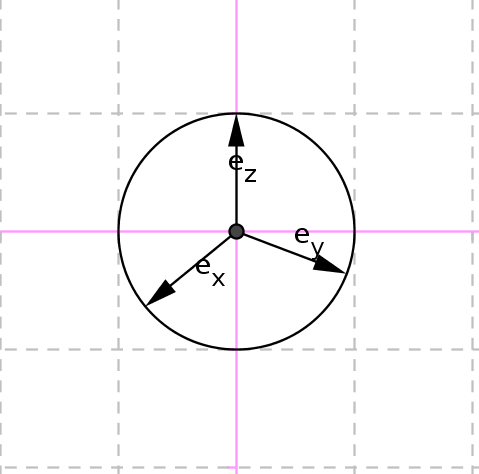
\includegraphics[scale=1]{unitvectors.png}
\caption{The three basis vectors point into the positive directions of the desired coordinate axes each. They are arranged around a circle with the trigonometric functions of cosine and sine. The coordinate system shown is a righthanded coordinate system.}
\end{figure}

\begin{figure}[ht]
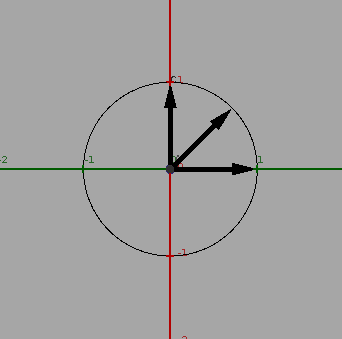
\includegraphics[scale=0.5]{lefthandbasis.png}
\caption{The three two dimensional basis vectors $\in \mathbb{R}^{2\times{3}}$ as a lefthanded coordinate system.}
\end{figure}


To reach all three (x,y) at the tips of the vectors, we will now pull out the cosine and sine functions and stuff them together
with $r$ and $\varphi$ into a 2x1 vector with two components. So any (x,y) on one line from the origin to far distance can be reached like in polar coordinates\footnote{Interested readers may find in \cite{Corral1}, \cite{Corral2} and \cite{Strang2} everything about polar coordinates, parametrization of x and y with cosine and sine, the unit circle and the distance or radius r and more to these topics.} with the following parametrization.\\

\begin{displaymath}
\left(\begin{array}{1}x\\y\end{array}\right) = \left(\begin{array}{1}r \cos \varphi\\ r \sin \varphi\end{array}\right)\\
\end{displaymath}\\

Which can alternativly be written like $(x,y) = (r \cos \varphi, r \sin \varphi)$.\\

Modeling the three two dimensional basis vectors with this information,
we get the following three two dimensional basis vectors. They point along the coordinate axes and are the ruler for our transformation.\\

\begin{displaymath}
\vec{e}_x := (r_x\cos(\varphi_x), r_x\sin(\varphi_x) )^T = \left(\begin{array}{1}r_x\cos(\varphi_x)\\r_x\sin(\varphi_x) \end{array}\right)\\
\end{displaymath}
\begin{displaymath}
\vec{e}_y := (r_y\cos(\varphi_y), r_y\sin(\varphi_y) )^T = \left(\begin{array}{1}r_y\cos(\varphi_y)\\r_y\sin(\varphi_y) \end{array}\right)\\
\end{displaymath}
\begin{displaymath}
\vec{e}_z := (r_z\cos(\varphi_z), r_z\sin(\varphi_z) )^T = \left(\begin{array}{1}r_z\cos(\varphi_z)\\r_z\sin(\varphi_z) \end{array}\right)\\
\end{displaymath}\\

Each component of (x,y,z) has now an own basis vector. By multiplying the cos terms for the x' and the sin terms for y' with the corresponding component of (x,y,z) and summing the three products up for each of x' and y', we directly obtain the right coordinate on the plane. All we would have to do is to connect the points again, or to fill the space between. 

\begin{figure}[ht]
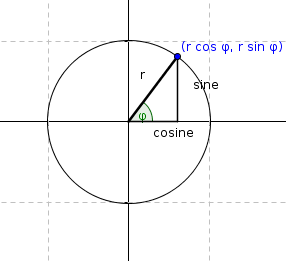
\includegraphics[scale=2]{unitcircle.png}
\caption{A picture of the unit circle, the hypotenuse r, the adjacent cosine, the opposite sine and the angle $\varphi$. It is a circle of radius r, and no longer the unit circle, if $r \neq 1$.}
\end{figure}

\subsection{About the vector basis lemma}\\

\subsubsection{The general formula like the Hamel Basis}

Remark. This section needs to be formulated again.\\

Remark II. Meanwhile i am sure, that Hamel-Basis is the right term to use here for the "generic formula". TODO.\\

I am talking about multiplying the coordinates with the new vector basis, which i state to be the same as the coordinate system we drew on a piece of paper at the beginning. We wrote down the angles, made out the unit length, and wrote down the three basis vectors with the information. Where is this coming from?\\

Every mathematics, physics or related course has a lesson, where the orthogonal basis of an object it's coordinate system is introduced. Orthogonality has some wonderful properties, and solving differential equations and other complicated systems take help from orthogonal vector sets.\\

A orthogonal basis is a set of 2 or three or up to infinite orthogonal or perpendicular vectors. They describe the coordinate system, the space, the dimensions, and one has to show for excercises, that the basis is linearly independent, that each basis vector points into it´s own dimension and not into the others.\\

Another excercise is to orthogonalize the existing vectors with Gram-Schmidt. \\

The one lemma we need is this general theorem for multiplying a vector with the a basis of a target coordinate system.\\

\begin{figure}
\begin{displaymath}
    \boldsymbol{E}_{\mathbb{R}^2} = \begin{pmatrix}1 & 0 \\ 0 & 1\end{pmatrix}    
\end{displaymath}
\caption{The standard basis for the $\mathbb{R}^{2}$ spans up the two dimensional space. The basis is true in $\mathbb{R}^{2\times{3}}$ but in $\mathbb{R}^{2}$ just a linear combination of $\lambda\begin{pmatrix}1\\0\end{pmatrix}$ and $\mu\begin{pmatrix}0\\1\end{pmatrix}$. }
\end{figure}

The plane gives us two possible directions, to go horizontal or vertical. And in a cartesian coordinate system with infinite points, we can choose any direction around a center point (x,y). Which is in the case of our coordinate system the origin at (0,0,0) or (0,0). We will see later, that the zero vector stays in the origin fo both systems.
Any not straight move will go horizontally or vertically by componentwise amounts. Any straight move horizontally or vertically will go by one of the components only.\\

\textbf{Remark} Edward was doing it right, then wrong (wrong with his pseudo-term). The basis is correct, but the space was $\mathbb{R}^{2\times{3}}$. In $\mathbb{R}^{2\times{3}}$ the basis can be shown. In R2 it is just a linear combination of three scalars with three vectors. I will be able to formulate this out in the next versions and have nice images for explanation in mind, which i will draw for.
\begin{figure}
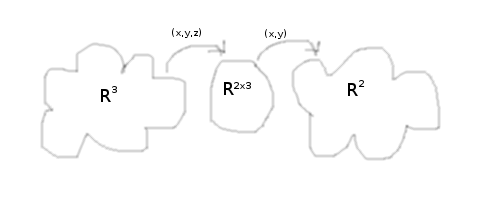
\includegraphics{mediator.png}
\caption{A temporary picture of the process. We multiply the 3-D points with the 2x3 matrix and get the 2-D points back.}
\end{figure}

The point is, the general formula holds with a 2x3 basis.

The basis acts as a middler beetween the two spaces. We walk through the $\mathbb{R}^{2\times{3}}$ when going from $\mathbb{R}^{3}$ to $\mathbb{R}^{2}.$\\

In $\mathbb{R}^{2}$ the basis is linearly dependent, and not a basis, but multiplying the coordinates with, yield the right image of the set of points processed. On the other side, in $\mathbb{R}^{2\times{3}}$ the basis can be explained, what i will do in the next versions. Have to read the text again, to catch my thread.\\

The formula for multiplying a vector with a base to get a new vector is this.\footnote{The formula can be found in many mathematics, chemistry and physics lecture scripts, and a good introduction is \cite{Strang1}.\\}

\begin{displaymath}
\vec{w} = \displaystyle\sum_{i=1}^{n} \vec{v}_{i}\vec{e}_{i}
\end{displaymath}

It is done componentwise for each row of the vector. $n$ is the number of the source dimensions. In our case it is $n = 3$. 
We are summing three products for each component of the new vector. Our old $\vec{v}$ is a $\vec{v} \in \mathbb{R}^3$.\\
With $\vec{v}_{i}$ as the coordinate component and $\vec{e}_{i}$ as the corresponding basis vector in the right component. 
$\vec{w}$ is the resulting new vector.  The new vector $\vec{w}$ is a $\vec{w} \in \mathbb{R}^2$.\\

In our scenario is $V \subseteq \mathbb{R}^{3}, \vec{v} \in V$ and $W \subseteq \mathbb{R}^{2}, \vec{w} \in W$.

\subsubsection{Connection to ijk-Notation}

This is also equal to

\begin{displaymath}
\vec{v} = x\vec{i} + y\vec{j} + z\vec{k}
\end{displaymath}

what also explains, what the ijk-Notation means. If you don´t use it already for determining determinants for
calculating cross products (\ref{crossproducts}). It is for describing a vector. Don´t forget, our $i, j, k$ basis is two dimensional, 
because we draw on a 2-D plane like the computer screen or a piece of paper. \\

With a 3x3 basis the vector $x\vec{i} + y\vec{j} + z\vec{k}$ is equal to \left(\begin{array}{1}x'\\y'\\z'\end{array}\right)$. But with a 2x3 basis the vector $x\vec{i} + y\vec{j} + z\vec{k}$ is becoming  \left(\begin{array}{1}x'\\y'\end{array}\right)$\\

\subsubsection{Coordinate system}

Remark. Needs to be formulated. New on July 23

The best i can do in the future editions of this text and for the concrete definition, is to say coordinate axes and coordinate system, without needing to know the horrible mathematic details, whose basis is used and whose not, and what words are right or wrong for.

The three vectors build the three coordinate axes of a three dimensional coordinate system in two dimensions. Nothing else.

The coordinates are transferred absolutely correct, they move along the vectors. They move the right units and only sidewards and upwards. The proportions are exact and can be controlled.

More rational is to say, a human designed this coordinate system and has put it right way round into the matrix, no matter how difficult another view of mathematics on the same vectors could become.

It is for the practical use, to use after plotting to project something 3-D onto the 2-D plane.


\subsection{Time to show the operation}

The operation of multiplying the (x,y,z) coordinate with our $\mathbb{R}^{2\times{3}}$ coordinate axis vectors in order is the following:\\

\begin{displaymath}
\left(\begin{array}{1}x'\\y'\end{array}\right) = \left(\begin{array}{1}
xr_x\cos\varphi_x + yr_y\cos\varphi_y + zr_z\cos\varphi_z\\
xr_x\sin\varphi_x + yr_y\sin\varphi_y + zr_z\sin\varphi_z\end{array}\right)\\
\end{displaymath}\\

Right, this small formula brings over the $\mathbb{R}^{2\times{3}}$ the unexpected images of the preimage from $R^3$ to $R^2$.\\

\begin{figure}[ht]
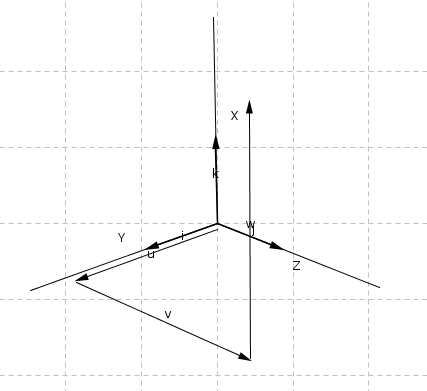
\includegraphics{pathcoords.png}
\caption{The path a point goes from the origin. Along the first axis, then from that parallel to the second along that axis, and last parallel to the third axis as many units as the coordinate says. You can not see on this picture, how it is deconstructed by cosine and sine into left and right moves. To see, just draw the two missing sides of the triangles under each move. The z axis has a cosine of 0. I will paint a new picture for.}
\end{figure}\\

It is almost time to finish the matrix and to go through a set of points to draw the new set of resulting points.
For this i close the explaining chapters and come to the part of the formal mathematical definitions.\\


\textbf{Remark.} \LaTeX and i are new to each other. For the theorems, proofs, defintions, corrolaries, examples there is the possibility of a personal layout.\\

\section{The $\mathbb{R}^{3} \rightarrow \mathbb{R}^{2}$ through $\mathbb{R}^{2\times{3}}$ transformation theorem}


Let $V$ be the set of all points $(x,y,z) \in V \subseteq R^3$ which are about to become transformed. $V := \{ \vec{v}=(x,y,z)^T | x,y,z \in \mathbb{R}, \vec{v} \in V \subseteq \mathbb{R}^{3} \}$.
Let $W$ be the set of all points $(x',y') \in W \subseteq R^2$ which are the result of the transformation $W ;= \{ \vec{w}=(x',y')^T | \vec{w} \in W \subseteq \mathbb{R}^{2} x',y' \in \mathbb{R}, \boldsymbol{A}\vec{v}=(x',y')\}$.\\

\textbf{Remark} study in progress.

Remark. What about the prime behind x and y. x', y' looks bad.

\subsection{The transformation matrix}

A $m\times n$ matrix is a rectangle or square of numbers.\\
\begin{displaymath}
    \boldsymbol{A} = (a_{ij})_{i,j \in \mathbb{N}^{+}} = \begin{pmatrix}a_{11} & ... & a_{mn}\\\vdots&\ddots&\vdots\\a_{m1} & ... & a_{mn}\end{pmatrix}
\end{displaymath}\\

Matrix multiplication, from left to right in the matrix and from top to bottom in the vector, and that row by row, is achived by \\

\begin{displaymath}
    \boldsymbol{A}\vec{v} = (\sum_{j=1}^{n}a_{ij}\vec{v}_{j})_{i = 1..m} = \begin{pmatrix}a_{11}v_{1} + a_{12}v_{2} + ... + a_{1n}v_n\\\vdots \\a_{m1}v_{1} + a_{m2}v_{2} + ... + a_{mn}v_n\end{pmatrix} = \left(\begin{array}{1}w_{1}\\\vdots\\w_{m}\end{array}\right) = \vec{w}

\end{displaymath}\\

This formula is not much different from the multiplication with a vector basis, but it also accounts for the rows in the formula. The vector basis multiplication implies the componentwise row operations by using vectors.\\

\index{Definition}
\newtheorem{Definition}{Definition}
\begin{Definition}

Let \boldsymbol{A} be the matrix containing the three, two dimensional and trigonometric, basis vectors in order, one each
column. You get a rectangular 2x3 matrix $\boldsymbol{A} \in \mathbb{R}^{2\times{3}}: \mathbb{R}^{3} \rightarrow \mathbb{R}^{2}$. With the basis vectors $\left(\begin{array}{1}r_{n} \cos \varphi_{n}\\r_{n} \sin \varphi_{n}\end{array}\right)$ in the three columns. \\

\begin{displaymath}
\boldsymbol{A} := \begin{pmatrix}
    \vec{e}_x & \vec{e}_y & \vec{e}_z
    \end{pmatrix}
    = 
    \begin{pmatrix}
    r_x\cos(\varphi_x) & r_y\cos(\varphi_y) & r_z\cos(\varphi_z) \\
    r_x\sin(\varphi_x) & r_y\sin(\varphi_y) & r_z\sin(\varphi_z) \\
    \end{pmatrix}
\end{displaymath}\\



$\boldsymbol{A}$ should be treated as operator $\boldsymbol{A} \in \mathbb{R}^{2\times{3}} : \mathbb{R}^3 \rightarrow \mathbb{R}^2$. $(\boldymbol{A})(\vec{x})=\boldsymbol{A}\vec{x}$, ($\vec{x}) \mapsto \boldsymbol{A}\vec{x}$. \\
\end{Definition}\\

Remark. Make this another definition.\\

The operator lives itself in L(V,W). L(V,W) contains all linear operators from V to W. A is mapping the input, which is 3-D from $V \subseteq \mathbb{R}^{3}$. onto the 2-D subset $W \subseteq \mathbb{R}^{2}$. The operator is NOT invertible due to a loss of one dimension and a lack of linear independence.\\

\textbf{Remark} This chapter needs to be overworked.

\subsection{The transformation}

\subsubsection{Matrix version}
\index{Theorem}
\newtheorem{Theorem}{Theorem (My fundamental theorem of transforming 3-D Points into 2-D Points)}
\begin{Theorem}\\
\label{Theorem}

If you multiply \boldsymbol{A}, the 2x3 matrix of the three two-dimensional basis vectors,
with the three-coordinate point $(x,y,z)$, the result is a two coordinate point, 
$(x',y')$. This point $(x',y')$ is the correct point on the two dimensional plane,
representing the point $(x,y,z)$ from the three dimensional coordinate system, you are transforming.\\

\begin{displaymath}
\boldsymbol{A}\left(\begin{array}{1}x\\y\\z\end{array}\right) = \left(\begin{array}{1}x'\\y'\end{array}\right)
\end{displaymath}

Applying the operator \boldsymbol{A} transforms the point $(x,y,z) \in V \subseteq \mathbb{R}^3$ into a new point $(x',y') \in W \subseteq \mathbb{R}^2$. 

\textbf{Proof}:\\

\begin{displaymath}
\boldsymbol{A}\left(\begin{array}{1}x\\y\\z\end{array}\right) = (\sum_{j=1}^{3}a_{ij}\vec{v}_{j})_{i=1,2}
%\end{displaymath}
%\beg{in{displaymath}
&= \left(\begin{array}{1}xr_x\cos(\varphi_x) + yr_y\cos(\varphi_y) + zr_z\cos(\varphi_z)\\
xr_x\sin(\varphi_x) + yr_y\sin(\varphi_y) + zr_z\sin(\varphi_z)\\
\end{array}\right) = \left(\begin{array}{1}x'\\y'\end{array}\right)
\end{displaymath}

\begin{figure}[ht]
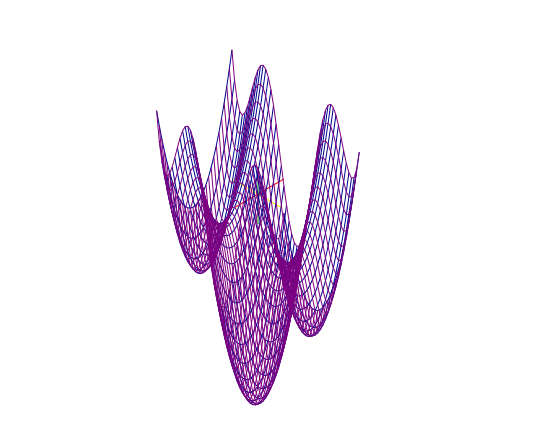
\includegraphics[scale=0.5]{fxyplot.png}
\caption{$f(x,y) = x^2 + y^2 + 3y \sin y$ from [-5,5] and [-3,3] on a Canvas2DRenderingContext}
\end{figure}
\end{Theorem}


\subsubsection{Vectorbasis version }

Remark. Under construction.

\begin{displaymath}
\vec{w} = \sum_{i=1}^{n}\vec{v}_{i}\vec{e}_{i}
\end{displaymath}

If you multiply the three-d vectors a linear dependet set of three two dimensional vectors, which represent the three coordinate axes on the plane with the formula of the Hamel-Basis, the resulting two dimensional vectors are the correct points on the plane.

Remark. A Hamel-Basis requires a linearly independent set of basis vectors, which we can not provide, due to the dimension change. I am still thinking about the right explainings. 

\begin{displaymath}
\vec{v} = (x,y,z)^{T}
\end{displaymath}
\begin{displaymath}    
\vec{w} = x\vec{e}_{x} + y\vec{e}_{y} + z\vec{e}_{z} \mbox{ which is equal to } x\vec{i} + y\vec{j} + z\vec{k} \\
\end{displaymath}    
\begin{displaymath}
    \vec{w} = \sum_{i=1}^{n}\vec{v}_{i}\vec{e}_{i} = \left(\begin{array}{1}xr_x\cos(\varphi_x) + yr_y\cos(\varphi_y) + zr_z\cos(\varphi_z)\\
xr_x\sin(\varphi_x) + yr_y\sin(\varphi_y) + zr_z\sin(\varphi_z)\\
\end{array}\right) = \begin{pmatrix}x'\\y'\end{pmatrix}
\end{displaymath}

TODO. 

\subsection{Computer implementations, left away the matrix, of the transformation}
\subsubsection{Generic computer code}

This should be in a border box.


\begin{example}
\fbox{
The following is example code for various computer systems.
}
\begin{lstlisting}
x_ = x*r*cos(alpha) + y*r*cos(beta) + z*r*cos(gamma)
y_ = x*r*sin(alpha) + y*r*sin(beta) + z*r*sin(gamma)
\end{lstlisting}\\
\fbox{ These are the one and only two lines of code you need.\\}

\end{example}\\


\subsubsection{JavaScript computer code}
\begin{example}
This is a full EcmaScript 6 snippet with all neccessary informations.\\
\begin{lstlisting}
let rad = (deg) => Math.PI/180*deg;
let r_x = 1, r_y = 1, r_z = 1; 
let phi_x = rad(220), phi_y = rad(330), phi_z = rad(90); 
let xAxisCos = r_x*Math.cos(phi_x), 
    yAxisCos = r_y*Math.cos(phi_y),
    zAxisCos = r_z*Math.cos(phi_z),
    xAxisSin = r_x*Math.sin(phi_x), 
    yAxisSin = r_y*Math.sin(phi_y),
    zAxisSin = r_z*Math.sin(phi_z);
let transform2d = ([x,y,z]) => [
    x*xAxisCos+ y*yAxisCos+ z*zAxisCos,
    x*xAxisSin+ y*yAxisSin+ z*zAxisSin];
let transform2dAll = (P) => P.map(transform2d);

let examplePoints = transform2dAll([[1,2,3], [3,4,5], [14,24,15]]);
\end{lstlisting}
\end{example}\\
\fbox{ This is the realistic amount of code to write to transform all points from 3-D to 2-D.\\}

\begin{figure}[ht]
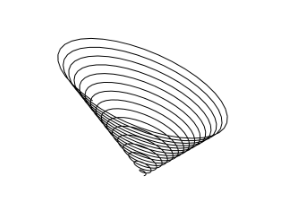
\includegraphics[scale=0.5]{conicalhelix.png}
\caption{A conical helix (t/2*Math.cos(t), t*Math.sin(t), t) shown as (x,y,z)=f(t) with implement.html on a Canvas2DRenderingContext testing the javascript example code.}
\end{figure}


\subsection{The transformation with functions, $f$ and $f \circ g$ version}

Remark. The first days, i could not see the forest, because of all these trees. 



The operation can be written as function, or as part of a composition of functions.\\

A big gain for this point transformation is the easy use to create surface plots and other functional graphs.\\

\subsubsection{As a function}

We begin with $f(\vec{x}) : V \subseteq \mathbb{R}^{3} \rightarrow \subseteq \mathbb{R}^{2}$.

$f(\vec{x})$ is mapping the three dimensional coordinates onto our designed coordinate system. The multiplication of the components with the horizontal and vertical displacements which are represented by the axes of our coordinate system is the fix content of our function. Assume we have the angles and units designed and the function is well defined for its purpose.

\begin{displaymath}
\label{f_function}
f(\vec{x}) := \left(\begin{array}{1}\vec{x}_{1}r_x\cos\varphi_x + \vec{x}_{2}r_y\cos\varphi_y + \vec{x}_{3}r_z\cos\varphi_z\\
\vec{x}_{1}r_x\sin\varphi_x + \vec{x}_{2}r_y\sin\varphi_y + \vec{x}_{3}r_z\sin\varphi_z\end{array}\right)
\end{displaymath}

\subsubsection{As a composition of the functions $f \circ g$}

There are various possibilities to combine the output of g and the input of f.

The following functions are compositions of two functions and take some input and return our 2-D points.

f is the transformation of the vector returned by g. g is taking the input in all examples and f is reworking the coordinates.

In other words, f is the same function as previously shown in \ref{f_function}..

Example 1. A call to $g(t)$ is returning a vector $\vec{v}$ passed to $f(\vec{x})$ by using the composition $f \circ g$ :  $f(g(t)) = \vec{w}$

\begin{center}
$g(t) : \mathbb{R} \rightarrow \mathbb{R}^{3}$\\
$f(\vec{x}) : \mathbb{R}^{3} \rightarrow \mathbb{R}^{2}$\\
\end{center}

See figure \ref{g_of_t_helix}

\begin{displaymath}
\label{g_of_t_code}
g(t) := \left(\begin{array}{1}t\times{\cos}t\\t\times{\sin}t\\t\end{array}\right)
\end{displaymath}

\begin{center}
\begin{figure}
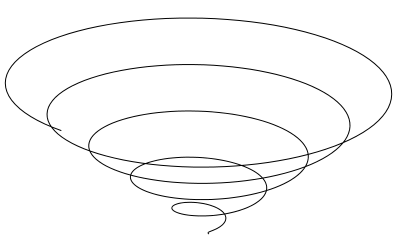
\includegraphics[scale=0.5]{conicalhelix2.png}
\label{g_of_t_helix}
\caption{Projected with the example javascript code is this an output of the function g(t) in \ref{g_of_t_code}.}
\end{figure}
\end{center}


Example 2. $g(x,y) = (x,y,z)^{T}$ which does not only produce z on x and y. It returns all three scalars together in one vector and passes that to our f.

\begin{center}
$g(x,y) : \mathbb{R}^{2} \rightarrow \mathbb{R}^{3}$\\
$f(\vec{x}) : \mathbb{R}^{3} \rightarrow \mathbb{R}^{2}$\\
\end{center}

Example. This function will give us a surface plot. See figure \ref{g_of_x_y_figure}

\begin{displaymath}
\label{g_of_x_y_code}
g(x,y) := \left(\begin{array}{1}x\\y\\\exp{-x^{2} - y^{2}}\end{array}\right)
\end{displaymath}

\begin{figure}
\label{g_of_x_y_figure}
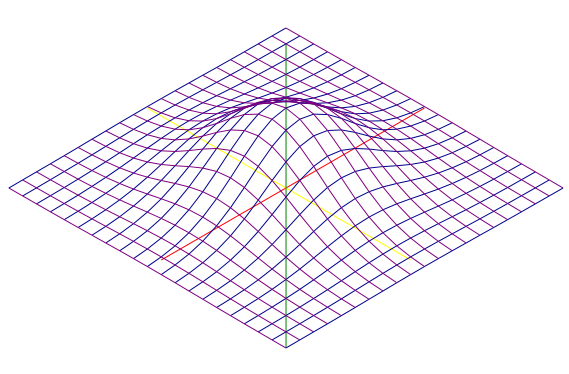
\includegraphics[scale=0.5]{expfunction.png}
\caption{This is $\exp -x^{2}-y{2}$ from \ref{g_of_x_y_code} plotted with the cheap3danimate.html code within $[-2,2] \times [-2,2]$.}
\end{figure}

Example 3. A $g(x,y,z)$ or $g(\vec{x})$ a three-d or vector-valued function returning a three-d vector.

\begin{displaymath}
\label{g_of_x_y_z_code}
g(x,y,z) := \left(\begin{array}{1}next\\next\\next\end{array}\right)
\end{displaymath}

The vector field.

\begin{center}
$g(\vec{x}) : \mathbb{R}^{3} \rightarrow \mathbb{R}^{3}$\\
$f(\vec{x}) : \mathbb{R}^{3} \rightarrow \mathbb{R}^{2}$\\
\end{center}

Remark. This list is longer. But it is 2 a.m. and i am stopping here.


\subsubsection{Differentiability}

Remark. This is under construction.

\subsubsubsection{Derivatives of \vec{f}(\vec{x}) : V \rightarrow W }

Again we begin with $\vec{f}(\vec{x}) : V \subseteq \mathbb{R}^{3} \rightarrow W \subseteq \mathbb{R}^{2}$.

\begin{displaymath}
\vec{f}(\vec{x}) := \left(\begin{array}{1}\vec{x}_{1}r_x\cos\varphi_x + \vec{x}_{2}r_y\cos\varphi_y + \vec{x}_{3}r_z\cos\varphi_z\\
\vec{x}_{1}r_x\sin\varphi_x + \vec{x}_{2}r_y\sin\varphi_y + \vec{x}_{3}r_z\sin\varphi_z\end{array}\right)
\end{displaymath}

The first derivatives after the vector are the following by using the product rule and partial differentiation. 
The scalar component of the input is gone, because the derivative is $1$ and the other summand of the derived product is zero, because the cosine or sine function are treated like either like a constant or like a function and become zero because there is the wrong variable to differentiate in the angle.\\

The derivatives of the angles are not taken. But it seems to be obvious, that the sin and cosine would be rotating around by 90 degrees each time the derivative of the derivative with respect to the angle is taken.\\

\begin{center}
\begin{displaymath}
\partial_{1}(\vec{f}(\vec{x})) = \vec{e}_{x}\\
\partial_{2}(\vec{f}(\vec{x})) = \vec{e}_{y}\\
\partial_{3}(\vec{f}(\vec{x})) = \vec{e}_{z}\\
\end{displaymath}
\end{center}

The second derivatives are already zero, because the returned vectors are constants with respect to the taken input variable.\
\begin{center}
\begin{displaymath}
\partial_{1}^{2}(\vec{f}(\vec{x})) = 0\\
\partial_{2}^{2}(\vec{f}(\vec{x})) = 0\\
\partial_{3}^{2}(\vec{f}(\vec{x})) = 0\\
\end{displaymath}
\end{center}



\section{Important proofs of the transformations behaviour}

Remark. This document is still under construction. 

A very important thing is to show, that the linearity of the transformation is in order. With a wrong function, bad thing can happen.
With the right functions, linear combinations should stay in the subspace.
\subsection{The origin stays in the origin}

A trivial proof is to prove, that the zero vector $\vec{0} \in \mathbb{R}^3$ maps to the zero vector $\vec{0} \in \mathbb{R}^2$.\\

\textbf{Proof}:
\begin{displaymath}
    \boldsymbol{A}\left(\begin{array}{1}0\\0\\0\end{array}\right)
    = \left(\begin{array}{1}0 + 0 + 0\\0 + 0 + 0\end{array}\right) 
    =\left(\begin{array}{1}0\\0\end{array}\right)
\end{displaymath}\\

\subsection{Points along one axis}

Another trivial proof is to prove, that coordinates lying on one axis are a multiple of the basis vector of the axis.\\

\textbf{Proof}:
\begin{displaymath}
    \boldsymbol{A}\left(\begin{array}{1}a\\0\\0\end{array}\right)
    = \left(\begin{array}{1}ar_x\cos \varphi_x + 0 + 0\\ar_x\sin \varphi_x  + 0 + 0\end{array}\right) 
    = a\vec{e}_x
\end{displaymath}

\begin{displaymath}
    \boldsymbol{A}\left(\begin{array}{1}0\\1\\0\end{array}\right)
    = \left(\begin{array}{1}0 + r_y\cos \varphi_y + 0\\0 + r_y\sin \varphi_y + 0\end{array}\right) 
    = \vec{e}_y
\end{displaymath}

\begin{displaymath}
    \boldsymbol{A}\left(\begin{array}{1}0\\0\\-b\end{array}\right)
    = \left(\begin{array}{1}0 + 0 - br_z\cos \varphi_z\\0 + 0 - br_z\sin \varphi_z\end{array}\right) 
    = -b\vec{e}_z
\end{displaymath}\\

\subsection{Multiplications with constants}

Another trivial proof is to show, that $\boldsymbol{A}(\lambda\vec{x}) = \lambda\boldsymbol{A}\vec{x}$. It doesn´t matter, where you multiply with the constant. You can multiply the original vector, or the resulting vector. You reach the same point.\\

\textbf{Proof}:\\
\begin{displaymath}
\begin{equation*}
\begin{align*}
\boldsymbol{A}(\lambda\vec{x}) &= \boldsymbol{A}\left(\begin{array}{1}\lambda{x}\\\lambda{y}\\\lambda{z}\end{array}\right)\\ &= \left(\begin{array}{1}\lambda{x}r_x\cos(\varphi_x) + \lambda{y}r_y\cos(\varphi_y) + \lambda{z}r_z\cos(\varphi_z)\\
\lambda{x}r_x\sin(\varphi_x) + \lambda{y}r_y\sin(\varphi_y) + \lambda{z}r_z\sin(\varphi_z)
\end{array}\right)\\
    &= \lambda\left(\begin{array}{1}xr_x\cos(\varphi_x) + yr_y\cos(\varphi_y) + zr_z\cos(\varphi_z)\\
xr_x\sin(\varphi_x) + yr_y\sin(\varphi_y) + zr_z\sin(\varphi_z)\\
\end{array}\right)\\
    &= \lambda\left(\begin{array}{1}x'\\y'\end{array}\right)\\
    &= \lambda\boldsymbol{A}\vec{x}
\end{align*}
\end{equation*}
\end{displaymath}\\


\subsection{Additions and subtractions}

Another trivial proof is to show, that $\boldsymbol{A}(\vec{v} + \vec{w}) = \boldsymbol{A}\vec{v} + \boldsymbol{A}\vec{w}$. 
It does not matter, if you add the original or the results . The outcome is the same point, the same vector.\\
 
\textbf{Proof}:\\

\begin{displaymath}
\begin{equation*}
\begin{align*}
\boldsymbol{A}\left(\begin{array}{1}x+u\\y+v\\z+w\end{array}\right) &= \left(\begin{array}{1}(x+u)r_x\cos(\varphi_x) + (y+v)r_y\cos(\varphi_y) + (z+w)r_z\cos(\varphi_z)\\
(x+u)r_x\sin(\varphi_x) + (y+v)r_y\sin(\varphi_y) + (z+w)r_z\sin(\varphi_z)\\
\end{array}\right)\\
            &= \left(\begin{array}{1}xr_x\cos(\varphi_x) + yr_y\cos(\varphi_y) + zr_z\cos(\varphi_z)\\
xr_x\sin(\varphi_x) + yr_y\sin(\varphi_y) + zr_z\sin(\varphi_z)\\
\end{array}\right) + \left(\begin{array}{1}ur_x\cos(\varphi_x) + vr_y\cos(\varphi_y) + wr_z\cos(\varphi_z)\\
ur_x\sin(\varphi_x) + vr_y\sin(\varphi_y) + wr_z\sin(\varphi_z)\\
\end{array}\right)\\    
    &= \left(\begin{array}{1}x'\\y'\end{array}\right) + \left(\begin{array}{1}u'\\v'\end{array}\right)\\
    &= \boldsymbol{A}\left(\begin{array}{1}x\\y\\z\end{array}\right) + \boldsymbol{A}\left(\begin{array}{1}u\\v\\w\end{array}\right)
\end{align*}
\end{equation*}
\end{displaymath}
\subsection{Rule of linearity}

\textbf{Corollary} From the previous two proofs, it is obvious to see, that
\begin{displaymath}
\boldsymbol{A}(\lambda\vec{v} + \kappa\vec{w}) = \lambda\boldsymbol{A}\vec{v} + \kappa\boldsymbol{A}\vec{w} = \lambda\left(\begin{array}{1}x'\\y'\end{array}\right) + \kappa\left(\begin{array}{1}u'\\v'\end{array}\right)\\
\end{displaymath}
which is a standard formulation of the rule of linearity. For example, you can find this rule in the form $\boldsymbol{A}(c\vec{x} + d\vec{y}) = c\boldsymbol{A}\vec{x} + d\boldsymbol{A}\vec{y}$ in \cite{Strang1}, but also in every linear algebra 1 lecture script.\\


\subsection{Convexity test}

Remark. Edward is new to convex sets. 

Convex sets contain the distance beetween two points inside the set. That means, that the direct way from a to be is not crossing the borders of the set. This can be imagined with real borders of a set. A round set, or a rectangle have all points inside together with their path. A star for example, where you have two points at two of the tips is not convex, the direct path, the straight line would cross the border of the star, leave the star, and reenter the star. There is a formula, which gives the points on the path.

\begin{displaymath}
u = \lambda\vec{x} + (1-\lambda)\vec{y}, \lambda \in [0,1], x,y \in V \implies u \in V
\end{displaymath}

The factor lambda lies beetween 0 and 1. If $\lambda = 0.1$ then is $(1-\lambda) = 0.9$, if $\lambda = 0.2$ then is $(1-\lambda) = 0.8$ and so on. The result is lying on the straight line of \vec{x} + \vec{y}. I have taken two vectors $\vec{x}, \vec{y} \in R^2$ and drawn them. After drawing the vector $\vec{x}+\vec{y}$ in the middle, i found 0.1 up to 0.9 lying on the line of the position vector to $\vec{x}+\vec{y}$.\\

Remark. Edward is new to convexity.

There is an inequality, which convex functions have to satisfy.

\begin{displaymath}
\|\lambda\vec{x} + (1-\lambda)\vec{y}\| \leq \lambda\|\vec{x}\| + (1-\lamda)\|\vec{y}\|
\end{displaymath}

or what expresses, that a function is convex.

\begin{displaymath}
f(\lambda\vec{x} + (1-\lambda)\vec{y}) \leq \lambda f(\vec{x}) + (1-\lamda)f(\vec{y})
\end{displaymath}

Our image is very precise, because we designed a real coordinate system. What is happening to our new vector? 

Remark. Edward is new to mathematics.

\begin{displaymath}
\lambda\boldsymbol{A}\vec{x} + (1-\lambda)\boldsymbol{A}\vec{y} = \boldsymbol{A}(\lambda\vec{x} + (1-\lambda)\vec{y})
\end{displaymath}

By the rule of linearity.

Remark. To be studied within the next days. One of the main theorems of fa is dealing with the convex sets. And the formula is ubiquitous like the sums of vector products. It makes sense to test this completly. 

\section{Convergence and Completeness}

\subsection{Neighborhood}

Remark. The first words are older than this position.

The neighborhood of a point (x,y,z) is a ball or a sphere with a radius r or \epsilon. The bowl or ball is complete, with inner points, the sphere just is the border of the ball. The bowl has the formula $B_{r}{ (x,y,z) : x^{2} + y^{2} + z^{2} <= r }$ and the sphere collects all points around with the radius of one $B_{r}(\vec{v}) :={ (x,y,z) : x^{2} + y^{2} + z^{2} = r }$.\\

Remark. This is under construction for the next versions.


\subsection{Cauchy Sequences}

Remark. These first words are older than this position.

Convergence: $\forall \epsilon > 0 \exists n_{0} \in N : \forall n \geq n_{0} \|u_{n}-u\| < \epsilon$ For every epsilon greater than 0 exists some starting point $n_{0}$ from which on the sequence items for any n greater than $n_{0}$ come closer together on each step. Means, the distance is getting smaller and smaller until the sequence converges to a point and the distance goes to zero.\\

A simpler proof is to show, that a converging sequence from $\mathbb{R}^{3}$ also converges, when being transformed to $\mathbb{R}^{2}$. \\


In three dimensions, all components of the sequence have to converge. It depends on your sequence, whether it returns a vector or is build by three sequences. Anyways, $(\vec{u}_{n})_{n \in \mathbb{N}^{+} }$ has to follow the ordinary rules, that $\lim_{n\rightarrow\infty}(\vec{u}_{n}) = \vec{v}$, or short, the sequence has to converge against the limit. $(\vec{u}_{n}) \rightarrow \vec{v}$


Remark. I have now to show, that the distance shrinks under epsilon and goes to zero, while the sequence goes to some point in space.
Together with the transformation in use on the resulting vector of the sequence. What will happen, seems to be obvious, but it is the must, to show.


Remark. This is under construction for the next Versions.


\section{Corollaries}

\subsection{Converting four Dimensions down to two dimensions}\\

The theorem can be used to handle more dimensions, for example can four two-dimensional
vectors represent a 4-D space on the 2-D plane. They get converted into the correct
2-D points. For Example, if you use a 2x4 matrix and convert all points at each 
instance of $t$ you have a moving object into the direction of the fourth basis vector. \\

\begin{displaymath}
\boldsymbol{A} := \begin{pmatrix}
    \vec{e}_x & \vec{e}_y & \vec{e}_z & \vec{e}_t\end{pmatrix}\\ = 
    \begin{pmatrix}
    r_x\cos(\varphi_x) & r_y\cos(\varphi_y) & r_z\cos(\varphi_z) & r_t\cos(\varphi_t)\\
    r_x\sin(\varphi_x) & r_y\sin(\varphi_y) & r_z\sin(\varphi_z) & r_t\sin(\varphi_t)\\
    \end{pmatrix}
\end{displaymath}

Here the basis is four times of two dimensions. A 2x4 matrix with four two dimensional basis vectors, one for each axis.\\

\begin{displaymath}
\boldsymbol{A}\left(\begin{array}{1}x\\y\\z\\t\end{array}\right) = \sum_{n} \vec{e}_{n}\vec{x}_{n} = \left(\begin{array}{1}x'\\y'\end{array}\right)\\
\end{displaymath}

\textbf{Proof}:

\begin{displaymath}
\boldsymbol{A}\left(\begin{array}{1}x\\y\\z\\t\end{array}\right) &= \left(\begin{array}{1}
xr_x\cos(\varphi_x) + yr_y\cos(\varphi_y) + zr_z\cos(\varphi_z) + zr_t\cos(\varphi_t)\\
xr_x\sin(\varphi_x) + yr_y\sin(\varphi_y) + zr_z\sin(\varphi_z)+ zr_t\sin(\varphi_t)\end{array}\right)\\
\end{displaymath}
\begin{displaymath}
&= x\vec{e}_x + y\vec{e}_y + z\vec{e}_z + t\vec{e}_t &= \sum_{n} \vec{e}_{n}\vec{x}_{n} &= \left(\begin{array}{1}x'\\y'\end{array}\right)
\end{displaymath}\\

The same method can be used, to convert points or vectors from any other number of dimensions, down to the $xy$-plane. It can also be used in a general m by n case.\footnote{http://de.wikipedia.org/wiki/Abbildungsmatrix, shows the m by n case.}

\subsection{Alternative definition of the transformation by using dot products}

Underways, i came to another conclusion. If i pull the two row vectors out of the matrix and define them as two column vectors,
then i can dot each with the coordinate vector and write the dot product into the component of the resulting vector.\\

\begin{displaymath}
    \vec{v} = \left(\begin{array}{1}x\\y\\z\end{array}\right)       \vec{c} = \left(\begin{array}{1}r_x\cos\varphi_x\\r_y\cos\varphi_y\\r_z\cos\varphi_z\end{array}\right)            \vec{s} = \left(\begin{array}{1}r_x\sin\varphi_x\\r_y\sin\varphi_y\\r_z\sin\varphi_z\end{array}\right)
\end{displaymath}
 
\begin{displaymath}
    \vec{w} = \left(\begin{array}{1}\vec{v}\cdot\vec{c}\\\vec{v}\cdot\vec{s}\end{array}\right)
\end{displaymath}

The result is $\vec{w} \in W$, $W \subseteq R^2$.\\

This can also be done with up to infinite dimensions which result in two coordinates then. Just add the dimensions to $\vec{v}, \vec{c}, \vec{s}$ and see.\\

\textbf{Proof}:

\begin{displaymath}
\left(\begin{array}{1}\vec{v}\cdot\vec{c}\\\vec{v}\cdot\vec{s}\end{array}\right) = \left(\begin{array}{1}
xr_x\cos(\varphi_x) + yr_y\cos(\varphi_y) + zr_z\cos(\varphi_z)\\
xr_x\sin(\varphi_x) + yr_y\sin(\varphi_y) + zr_z\sin(\varphi_z)\end{array}\right) = \left(\begin{array}{1}x'\\y'\end{array}\right)
\end{displaymath}


\subsection{Orthogonality in the 2x3 matrix}

\textbf{Remark. This is an assumption. Proof follows.}

I think this is more about the right angle in the two dimensions and the linear combination of the three input values, once for each direction of the right angle here. It is still the 3-D on 2-D coordinate system with image and it should do exactly that.\\

Probably already found. 2-D (in each column, the two rows) mapping orthogonal, 3-D is linear (three moves left-right, three up-down) in the 2x3. In the 3x2 case the converse. Do never forget, that cos and sin are $\perp$ and form a right angle. TODO.\\

I mean. In each of the three column vectors, the map to the plane is defined by orthogonality of the two rows. Even if we change
from the perpendicular sine and cosine to some weird numbers, it would be interpreted as x and y and depend on the base used in the R2.\\





\section{Summary}

\subsection{Summary of all neccessary steps}
\begin{enumerate}
\item Lay out the three basis vectors around a circle and write down the angles $\varphi_{n}$. Programmers have to write down a variable for anyways.
\item Write down the basis vectors $\vec{e}_{n}$ as $r_{n} \cos \varphi_{n}$ and $r_{n} \sin \varphi_{n}$ (two dimensional). Don´t multiply with $r_{n}$ for a unit length of $1$ or multiply with $r_{n}$ to change the length of the basis vector.
\item Put the three basis vectors $\vec{e}_{n}$ into a matrix \bigsymbol{A}. Programmers can directly code the two lines of multiplication and forget the formal rest.
\item Iterate over your points and multiply each $(x,y,z)$ with the matrix \boldsymbol{A}, which acts as a linear operator, and put $(x',y')$ into your new set.\footnote{Alternativly you can use the dot product to dot $(x,y,z)$ with the cosine vector for x' and dot $(x,y,z)$ with the sine vector for y'. The calculation is identical then.}
\end{enumerate}

\textbf{Remark}\\
About the word \emph{unit}. I am not really sure, if i have to use \emph{base vector} for a vector of any length and \emph{unit vector} only for the \emph{unit length} of $1$. Because of the misleading mismatch with the \emph{unit} of the thought \emph{coordinate axes}, which the \emph{base vector} defines, i tend in the first versions to misuse the word \emph{unit vector} for both. If you find this, or any other formal mistake, be sure, it is not wanted :-) I will try to remove more of these spelling errors\footnote{The \emph{Gerholdian operator}, the \emph{Gerholdian basis}, the \emph{Gerhold projection matrix}, the \emph{Gerhold transformation} are my favourite nicknames for my late discovery, making sure, the three two dimensional and trigonometric basis vectors, which i explained, sit in the matrix.} in the next versions.
\section{Glossary}

I am nativly a german speaking man. To reduce the risk of misunderstanding me, i will write down the terms, which i use in this document. So you can read from my definition, what i mean with and decide by yourself, what´s the correct word, i wanted to use.\\

Remark. This doesnt contain the right info. I should use basis and coordinate axes interchangably, but i use other words.

\begin{tabular}{-l-l-l}
    assumed english & german & personal definition \\

\hline
    basis &     Basis &     A system of vectors, with which any coordinate has to be transformed.\\
    & & A basis transforms your coordinates into your desired coordinate system.\\
    & & A basis is regularly a set of linearly independent vectors. They span the space.\\    
    & & For example are $(1,0)$ and $(0,1)$ the basis for the $\mathbb{R}^{2}$ and\\
    & & $(3,4)$ is a combination of $3\times(1,0)$ and $4\times(0,1)$,\\
    & & The basis is also synonymous for the coordinate axes.\\

\hline    
    vector, point, coordinate & Vektor, Punkt, Koordinate & A vector has a length and a direction. \\
    & & The tails of the vectors here meet in the origin. The point is the tip\\
    & & of the vector, or the word for the coordinates in the cartesian system. \\
    & & The words point, vector, coordinate are used interchangably in this text and depend \\
    & & on what your numbers mean.\\
\hline 
    component & Komponente & A component of a vector or a matrix or a point is one of the scalars
    inside. For a (x,y,z) Vector, x is a component.\\

\hline 
    operator & Operator & A matrix is a linear map or a linear operator. The former is linear algebra\\
    & & and the latter is functional analysis. Well, a better application for the transformation is to visualize\\
    & & both, so both should be used. But possibly i currenly intermingle these words a bit, trying to find the right.\\
    & & The definition of the 2x3 operator is not complete, it is for example not invertible, has no determinant, \\
    & & looses the third dimensions also, when restoring, with say least squares, \\

\end{tabular}

\textbf{Remark} incomplete.

\appendix

\section{Deconstructing and proving the 2x3 basis }

\subsection{2x3 standard basis}

A 2x3 basis is a set of six matrices being constructed out of five basis vectors. In the Appendix of \cite{Strang1}, there is a basis of a 2x3 matrix printed, together with a few arguments. The professor constructed a 2x3 standard basis by multiplying the 2-D standard basis vectors with the 3-D standard vectors.\\

\begin{displaymath}

\begin{center}
e_{1}^{\mathbb{R}^{2}} = \begin{pmatrix}1\\0\end{pmatrix}
e_{2}^{\mathbb{R}^{2}} = \begin{pmatrix}0\\1\end{pmatrix}\\

e_{1}^{\mathbb{R}^{3}} = \begin{pmatrix}1\\0\\0\end{pmatrix}
e_{2}^{\mathbb{R}^{3}} = \begin{pmatrix}0\\1\\0\end{pmatrix}
e_{2}^{\mathbb{R}^{3}} = \begin{pmatrix}0\\0\\1\end{pmatrix}

\end{center}
\end{displaymath}

Multiplying $e_{i}^{\mathbb{R}^{2}}$ with $(e_{j}^{\mathbb{R}^{3}})^{T}$ yields six independent matrices, which, when added, form the standard basis.

\begin{displaymath}
E^{\mathbb{R}^{2\times{3}}} =
\begin{pmatrix}1&0&0\\0&0&0\end{pmatrix}+
\begin{pmatrix}0&1&0\\0&0&0\end{pmatrix}+
\begin{pmatrix}0&0&1\\0&0&0\end{pmatrix}+
\begin{pmatrix}0&0&0\\1&0&0\end{pmatrix}+
\begin{pmatrix}0&0&0\\0&1&0\end{pmatrix}+
\begin{pmatrix}0&0&0\\0&0&1\end{pmatrix}

\end{displaymath}

My task is now, to deconstruct our formula, to meet the requirements. 

\begin{displaymath}
\begin{center}
e_{1}^{\mathbb{R}^{2}} = \begin{pmatrix}u\\0\end{pmatrix}
e_{2}^{\mathbb{R}^{2}} = \begin{pmatrix}0\\v\end{pmatrix}\\
e_{1}^{\mathbb{R}^{3}} = \begin{pmatrix}a\\0\\0\end{pmatrix}
e_{2}^{\mathbb{R}^{3}} = \begin{pmatrix}0\\b\\0\end{pmatrix}
e_{2}^{\mathbb{R}^{3}} = \begin{pmatrix}0\\0\\c\end{pmatrix}\\
E^{\mathbb{R}^{2\times{3}}} =
\begin{pmatrix}ua&0&0\\0&0&0\end{pmatrix}+
\begin{pmatrix}0&ub&0\\0&0&0\end{pmatrix}+
\begin{pmatrix}0&0&uc\\0&0&0\end{pmatrix}+
\begin{pmatrix}0&0&0\\va&0&0\end{pmatrix}+
\begin{pmatrix}0&0&0\\0&vb&0\end{pmatrix}+
\begin{pmatrix}0&0&0\\0&0&vc\end{pmatrix}
\end{center}
\end{displaymath}
Here we can subtitute
\begin{displaymath}
ua=r_x\cos\varphi_x,
va=r_x\sin\varphi_x,
ub=r_y\cos\varphi_y,
vb=r_y\sin\varphi_y,
uc=r_z\cos\varphi_z,
vc=r_z\sin\varphi_z,
\end{displaymath}
It should result in
\begin{displaymath}
\begin{center}
\begin{pmatrix}r_x\cos\varphi_x&0&0\\0&0&0\end{pmatrix}+
\begin{pmatrix}0&r_y\cos\varphi_y&0\\0&0&0\end{pmatrix}+
\begin{pmatrix}0&0&r_z\cos\varphi_z\\0&0&0\end{pmatrix}+\\
\begin{pmatrix}0&0&0\\r_x\sin\varphi_x&0&0\end{pmatrix}+
\begin{pmatrix}0&0&0\\0&r_y\sin\varphi_y&0\end{pmatrix}+
\begin{pmatrix}0&0&0\\0&0&r_z\sin\varphi_z\end{pmatrix}\\
   = \begin{pmatrix}
    r_x\cos\varphi_x & r_y\cos\varphi_y & r_z\cos\varphi_z \\
    r_x\sin\varphi_x & r_y\sin\varphi_y & r_z\sin\varphi_z \\
    \end{pmatrix}
\end{center}
\end{displaymath}

Remark. My first conclusions, while inventing the chapter and the excercise. To be removed.

From trigonometry, we know, that cosine and sine form a right angle. They are perpendicular to each other. But taking the norm of the vector results in r, not in 0, because $sin^{2}+cos^{2}=1$. $r sin^{2}+r cos^{2}=r^{2}$. This is not orthogonal in terms of the dot product, which should result in 0, if the angle is 90 degrees.\\

For simplification we should do a few things. First, we assume $r_x = r_y = r_z = 1$. Without a factor in front of sine and cosine, they both together have unit length of one. With $\|\begin{pmatrix}\frac{r_x\cos\varphi_x}{r_x}\\\frac{r_x\sin\varphi_x}{r_x}\end{pmatrix}\| = 1$ the vector is normalized. \\

Secondly, we substitute the cosine and sine terms with simple letters. Sine, cosine and r form a triangle. Thinking of a triangle, and sin = opposite/hypotenuse and cos = adjacent/hypotenuse, will make it easier for us to find the factors and to solve this system.\\

\begin{displaymath}
    cos = \frac{adjacent}{hypotenuse} 
    sin = \frac{opposite}{hypotenuse}
\end{displaymath}

\textbf{Remark}. Today i prepared this decomposition.\\

Remark. I think, this can be also done with Gram-Schmidt. Gram-Schmidt is an iterative process, to reduce the first vector, then with the information the second and so on. But i have not tried it since my first excercise with. \\

\subsection{Lefthands and righthands}

Without calculating them, but concluding them from the existing, i get the following matrices, which look like bases, containing only zeros and ones.

\begin{displaymath}
    E^{\mathbb{R}^{2\times{3}}}_{lefthand} = \begin{pmatrix}1&0&1\\0&1&1\end{pmatrix}
\end{displaymath}
\begin{displaymath}
    E^{\mathbb{R}^{2\times{3}}}_{righthand} = \begin{pmatrix}-1&1&0\\-1&-1&1\end{pmatrix}
\end{displaymath}

\textbf{Remark} Proof or contradictions TODO

\section{Proving more rules of vector spaces}\\

Remark. The linearity proofs should go together with the formula in the main part about.

Remark. The remainder will be reordered and is TODO.

\subsection{Dot product}

The dot product, scalar product or inner product is the sum of the vector component products. $(\vec{v}, \vec{w})$ is $\sum_{i=1}^{n}\vec{v}_{i}\vec{w}_{i}$.  \\

$\sum_{i=1}^{n}\vec{v}_{i}\vec{w}_{i} = 0$ means, that $\vec{v} \perp \vec{w}$ \\

The basis formula is this

\begin{displaymath}
    (v,w) = \sum_{i=1}^{n}\vec{v}_{i}\vec{w}_{i}
\end{displaymath}

A product with the zero vector.

\begin{displaymath}
    (\vec{0},w) = \sum_{i=1}^{n}\vec{0}_{i}\vec{w}_{i} = 0
\end{displaymath}

Linear combinations.

\begin{displaymath}
    (\lambda\vec{v},\vec{w}) = \sum_{i=1}^{n}\lambda\vec{v}_{i}\vec{w}_{i}
    = \lambda\sum_{i=1}^{n}\vec{v}_{i}\vec{w}_{i} = \lambda(\vec{v}, \vec{w})
\end{displaymath}

\begin{displaymath}
    (\lambda\vec{v},\vec{w}+\vec{x}) = \sum_{i=1}^{n}\lambda\vec{v}_{i}(\vec{w}_{i}+\vec{x}_{i})
    = \lambda(\sum_{i=1}^{n}\vec{v}_{i}\vec{w}_{i}+\sum_{i=1}^{n}\vec{v}_{i}\vec{x}_{i})
    = \lambda((\vec{v},\vec{w})+(\vec{v},\vec{x}))
\end{displaymath}

\begin{displaymath}
    (\lambda\vec{v},\kappa\vec{w}) = \sum_{i=1}^{n}\lambda\vec{v}_{i}\kappa\vec{w}_{i}
    = \lambda\kappa\sum_{i=1}^{n}\vec{v}_{i}\vec{w}_{i} = \lambda\kappa(\vec{v}, \vec{w})
\end{displaymath}

\begin{displaymath}
\begin{center}
    (\lambda\vec{v}+\mu\vec{x},\kappa\vec{w}+\nu\vec{y})\\
    = \sum_{i=1}^{n}(\lambda\vec{v}_{i}+\mu\vec{x}_{i})(\kappa\vec{w}_{i}+\nu\vec{y}_{i})\\
    = (\lambda\vec{v},\kappa\vec{w}) + (\lambda\vec{v},\nu\vec{y}) + (\kappa\vec{w},\mu\vec{x}) + (\kappa\vec{w},\nu\vec{y})\\
    = \lambda(\kappa(\vec{v},\vec{w}) + \nu(\vec{v},\vec{y})) + \kappa(\mu(\vec{w},\vec{x}) + \nu(\vec{w},\vec{y}))\\
\end{center}    
\end{displaymath}

\subsection{The cross product}\label{crossproducts}

\begin{displaymath}
\begin{pmatrix}
    \vec{i} & \vec{j} & \vec{k}\\
    a_1 & a_2 & a_3\\
    b_1 & b_2 & b_3
\end{pmatrix} =
\begin{vmatrix}
a_2 & a_3 \\
b_2 & b_3 
\end{vmatrix} \vec{i} - \begin{vmatrix}a_1 & a_3\\ b_1 & b_3\end{vmatrix} \vec{j} + \begin{vmatrix}a_1 & a_2\\b_1 & b_2\end{vmatrix} \vec{k} = \left(\begin{array}{1}c_1\\c_2\\c_3\end{array}\right)
\end{displaymath}

You write a new vector $x\vec{i}-y\vec{j}+z\vec{k}$ (pay attention to the minus) with the determinants, which you obtain by scratching current column and the first row. You multiply the determinant with i, j, or k.Which

\begin{displaymath}
    \vec{a} \times \vec{b} = (a_{2}b_{3}-a_{3}b_{2})\vec{i} - (a_{1}b_{3}-a_{3}b_{1})\vec{j} + (a_{1}_b{2}-a{2}b_{1})\vec{k} = \vec{c}
\end{displaymath}

If the cross product does not yield a new vector, but the \vec{0} zero vector, the two vectors are not on the same plane.

\subsection{Normal vectors}

Are perpendicular to the surface and give the orientation.

\subsection{About the norm}

\subsubsection{Vector norms}

The norm is the word for the vector length. Or better, it is the multidimensional \emph{absolute value} of a vector. Remember from single variable calculus that $|-x|=x$ and $|x|=x$. The norm kind of does this with all values and puts them together.\\

Remark. Please write these explanations again, Edward..

The norm used is the euclidean norm, or the 2-norm. This is the square root of the sum of the squares of the absolute values of the components $\|\vec{x}\| = \sqrt{\sum_{i=1}^{n}|x_{i}|^2}$. In linear algebra, functional analysis and topology lectures there are three fundamental properties of the norm repeating. Definiteness, homogenity and the triangle inequality.\\

\textbf{Definitness} Show that $\|\vec{x}\| = 0 \iff \vec{x} = 0$\\

\begin{displaymath}
    \|\vec{x}\| = \|\vec{0}\| = \sqrt{0^{2} + 0^{2}} = 0
\end{displaymath}\\

\textbf{Homogenity} Show that $\|a\vec{x}\| = |a|\|\vec{x}\|$\\
\begin{displaymath}
    \|a\vec{x}\| = \sqrt{|a\vec{x}_1|^{2} + |a\vec{x}_2|^{2}} = \sqrt{|a|^{2}(|\vec{x}_1|^{2} + |\vec{x}_2|^{2})} = |a|\sqrt{|\vec{x}_1|^{2} + |\vec{x}_2|^{2}} = |a|\|\vec{x}\|
\end{displaymath}\\

\textbf{Triangle inequality} Show that $ \|\boldsymbol{A}(\vec{v} + \vec{w})\| \leq \|\boldsymbol{A}\vec{v}\| + \|\boldsymbol{A}\vec{w}\|$\\

This means, the path over two sides of the triangle is longer, than the side left over, no matter which way you turn. And it is a triangle, because the three points in the space are by at least one unit.

\begin{displaymath}
    \sqrt{\sum_{i=1}^{n}|\vec{v}_{i} + \vec{w}_{i}|^{2}} \leq \sqrt{\sum_{i=1}^{n}|\vec{v}_{i}|^{2}} + \sqrt{\sum_{i=1}^{n}|\vec{w}_{i}|^{2}} 
\end{displaymath}\\

Ok here we go again.

\begin{displaymath}
(\vec{v}+\vec{w}, \vec{v}+\vec{w})^{\frac{1}{2}} \leq (\vec{v},\vec{v})^{\frac{1}{2}}+(\vec{w},\vec{w})^{\frac{1}{2}}
\end{displaymath}

 This time i tried it algebraically, to first remove the root by squaring both sides. 

\begin{displaymath}
(\vec{v}+\vec{w}, \vec{v}+\vec{w}) \leq (\vec{v},\vec{v}) + 2(\vec{v},\vec{v})^{\frac{1}{2}}(\vec{w},\vec{w})^{\frac{1}{2}} + (\vec{w},\vec{w})
\end{displaymath}
Written as sum this is

\begin{displaymath}
\sum_{i=1}^{n}\vec{v}_{i}^{2}+2\vec{v}_{i}\vec{w}_{i}+\vec{w}_{i}^{2} \leq \sum_{i=1}\vec{v}_{i}^{2}+2(\sum_{i=1}^{n}\vec{v}_{i}\vec{v}_{i})^{\frac{1}{2}}(\sum_{i=1}^{n}\vec{w}_{i}\vec{w}_{i})^{\frac{1}{2}}+\sum_{i=1}^{n}\vec{w}_{i}^{2}
\end{displaymath}

This can be simplified. Now assume i split the left side up into three sums. And for more simplification i leave the equal (v,v) and (w,w) on both sides away, since they are summed, not multiplied. We get

\begin{displaymath}
2(\vec{v},\vec{w}) \leq 2(\vec{v},\vec{v})^{\frac{1}{2}}(\vec{w},\vec{w})^{\frac{1}{2}}
\end{displaymath}

Now i square it again to get rid of the square roots, and compare finally.

\begin{displaymath}
4(\vec{v}, \vec{w})^{2} \leq 4(\vec{v},\vec{v})(\vec{w},\vec{w}) 
\end{displaymath}

Which is 

\begin{displaymath}
4\sum_{j=1}^{n}\sum_{i=1}^{n}\vec{v}_{i}\vec{w}_{j} \leq 4\sum_{j=1}^{n}\sum_{i=1}^{n}\vec{v}_{i}^{2}\vec{w}_{j}^{2}
\end{displaymath}

Remark. When reading myself, i am sure, this last step is wrong, and the two vectors left have to be squared, too. I will calculate that again and correct then.\\


\textbf{Cauchy-Schwarz inequality} There is another interesting inequality.

TODO\\

\begin{displaymath}
    |\vec{v}\cdot\vec{w}|^{2} \leq \|\vec{v}\|^{2}\|\vec{w}\|^{2}
\end{displaymath}

The absolute value of the dot product squared is less or equal to the product of the two norms squared. Squaring the two norms to the right cancels the outer square root on the norms away, so that you multiply with the full vector length squared. So both sides are squares. Left is the dot product of the two vectors squared, on the right side the squared lengths of the two vectors are multiplied. So which square or rectangle is larger? You know by the formula anyways.

\begin{displaymath}
    |\sum_{i=1}^{n}\vec{v}_{i}\vec{w}_{i}|^{2} \leq ((\sum_{i=1}^{n}|\vec{v}_{i}|^{2})^{\frac{1}{2}})^{2}((\sum_{i=1}^{n}|\vec{w}_{i}|^{2})^{\frac{1}{2}})^{2}\\
\end{displaymath}
\begin{displaymath}
|\sum_{i=1}^{n}\vec{v}_{i}\vec{w}_{i}|^{2} \leq ((\sum_{j=1}^{n}\sum_{i=1}^{n}|\vec{v}_{i}|^{2}|\vec{w}_{i}|^{2})^{\frac{1}{2}})^{2} 
=
|\sum_{i=1}^{n}\vec{v}_{i}\vec{w}_{i}|^{2} \leq \sum_{j=1}^{n}\sum_{i=1}^{n}(|\vec{v}_{i}||\vec{w}_{i}|)^{2}
\end{displaymath}



\textbf{Remark} This subsection is not complete. And may contain mistakes.\\

\textbf{Remark} If i am reading right, it contains really a mistake. In the middle.

\subsubsection{Matrix norms}

There are a few possible ways to measure the multidimensional absolute values of a matrix.

Row wise. Sum up each row vector, and return the largest. This is the row norm.

\begin{displaymath}
\|A\|_{row} = \max_{i=1..n} { \sum_{j=1} |A_{ij}| }
\end{displaymath}

Column wise. Sum up each column vector, and return the largest. This is the column norm.


\begin{displaymath}
\|A\|_{column} = \max_{j=1..n} { \sum_{i=1} |A_{i}j| }
\end{displaymath}


\subsubsection{Operator norms}

The operatornorm is a dependent norm. It depends on the currently used norm. 

\begin{displaymath}
\|A\| = \|\phi\| := \sup\{ \phi(\vec{x}) : \|x\|=1 \}
\end{displaymath}

Remark. This is by heart. But i sure i am not through with using it correctly.


\subsection{Parallelogram equation}

\begin{displaymath}
2(\|v\|^{2} + \|w\|^{2}) = \|v+w\|^{2}+\|v-w\|^{2}
\end{displaymath}

This equation says, that the square sum of the parallelogram equals the square sum of the four sides.\footnote{This is a direct translated cite from a lecture script. http://pages.math.tu-berlin.de/~ferus/skripten.html from Lineare Algebra I.}\\


\textbf{Proof}:
\begin{displaymath}
2(\sum_{i=1}^{n}\vec{v}_{i}^{2} + \sum_{i=1}^{n}\vec{w}_{i}^{2}) = \sum_{i=1}^{n}\vec{v}_{i}^{2}+2\vec{v}_{i}\vec{w}_{i}+\vec{w}_{i}^{2}+\vec{v}_{i}^{2}-2\vec{v}_{i}\vec{w}_{i}+\vec{w}_{i}^{2} = \sum_{i=1}^{n}2\vec{v}_{i}^{2}+2\vec{w}_{i}^2 = 2\sum_{i=1}^{n}\vec{v}_{i}^{2}+\vec{w}_{i}^{2} = 2(\sum_{i=1}^{n}\vec{v}_{i}^{2} + \sum_{i=1}^{n}\vec{w}_{i}^{2})
\end{displaymath}




\subsection{Normalizing a vector}

If you wish to take the length of the vector, you take the norm $\|\vec{v}\|_{V}$ in three dimensions or $\|\vec{w}\|_{W}$ in two dimensions. If you wish to reduce or enlarge a vector to unit length, that $\|\vec{v}\|=1$ or $\|\vec{w}\|=1$, you can do this, by updating the or creating a new vector, by dividing the old vector components through the old vectors length. Taking the norm then, results in 1.\\

\begin{displaymath}
    \vec{w}_{normalized} = \frac{\vec{w}}{\|\vec{w}\|} \implies \|\vec{w}_{normalized}\| = 1
\end{displaymath}

\textbf{Proof}:

\begin{displaymath}
\vec{w}  = \left(\begin{array}{1}a\\b\end{array}\right)
\end{displaymath}
\begin{displaymath}
    \|\left(\begin{array}{1}a\\b\end{array}\right)\| = \sqrt{a^{2}+b^{2}}\\
\end{displaymath}
\begin{displaymath}
    \vec{w}_{normalized} = \frac{\vec{w}}{\|\vec{w}\|} 
    = \left(\begin{array}{1}\frac{a}{\sqrt{a^{2}+b^{2}}}\\\frac{b}{\sqrt{a^{2}+b^{2}}}\end{array}\right)
\end{displaymath}
\begin{displaymath}
    \|\vec{w}_{normalized}\| = \sqrt{\left(\frac{a}{\sqrt{a^{2}+b^{2}}}\right)^{2}+\left(\frac{b}{\sqrt{a^{2}+b^{2}}}\right)^{2}} = \sqrt{\frac{a^{2}+b^{2}}{a^{2}+b^{2}}} = \sqrt{1} = 1
\end{displaymath}



\subsection{Metrics}

Where a norm is, there will be a metric induced.
The measurement of the distance between two points is defined by the d-function. It is the length of the difference vector between the two points.\\

\begin{displaymath}
    d(\vec{x}, \vec{y}) = \|\vec{x}-\vec{y}\| = \sqrt{\sum_{i=1}^{n}|\vec{x}_{i}-\vec{y}_{i}|^2}
\end{displaymath}

Metrics have three fundamental properties.
\begin{enumerate}
\item If the distance is zero, the vectors are equal.
\begin{displaymath}
d(x,y) = 0 \iff x = y
\end{displaymath}
\item It does not matter, whether you read $d(x,y)$ or $d(y,x)$, the number must be equal. The absolute value function $|\pm n| = n, \pm n \in \mathbb{Q}$ makes sure
\begin{displaymath}
d(x,y) = d(y,x)
\end{displaymath}
\item The third one is the triangle inequality. Going over another point is always a step longer.
\begin{displaymath}
d(x,z) \leq d(x,y) + d(y,z) 
\end{displaymath}
\end{enumerate}


\textbf{Remark} This subsection is not complete and has to be continued. The plan is to measure or estimate now the differences between the original coordinates and the new planar coordinates. 

\subsection{Transpose and TODO}

A 2x3 matrix also has a transpose. Multiplying both result in two different square matrices. $\boldsymbol{A}^T\boldsymbol{A}$ is a 3x3 matrix. And $\boldsymbol{A}\boldsymbol{A}^T$ is a 2 by 2 matrix.\\

\begin{displaymath}
\left(
    \begin{array}{111}
    r_x\cos(\varphi_x) & r_y\cos(\varphi_y) & r_z\cos(\varphi_z) \\
    r_x\sin(\varphi_x) & r_y\sin(\varphi_y) & r_z\sin(\varphi_z) \\
    \end{array}
\right)^T
= \left(
    \begin{array}{11}
    r_x\cos(\varphi_x) & r_x\sin(\varphi_x)\\
    r_y\cos(\varphi_y) & r_y\sin(\varphi_y)\\
    r_z\cos(\varphi_z) & r_z\sin(\varphi_z) \\
    \end{array}
\right)
\end{displaymath}\\

Multiplying out the transposes yield the following forms.\\

$\boldsymbol{A}\boldsymbol{A}^T$, a 2 by 2 matrix.\\

\begin{displaymath}
\boldsymbol{A}\boldsymbol{A}^T = \begin{pmatrix} 
\sum_{i=1}^{3}r_{n}^2\cos^{2}\varphi_{n} & \sum_{i=1}^{3}r_{n}^2\cos\varphi_{n}\sin\varphi_{n}\\
\sum_{i=1}^{3}r_{n}^2\cos\varphi_{n}\sin\varphi_{n} & \sum_{i=1}^{3}r_{n}^2\sin^{2}\varphi_{n}
\end{pmatrix} = \begin{pmatrix}a & b\\b & c
\end{pmatrix}

In the 2x2 matrix $\boldsymbol{A}\boldsymbol{A}^T$ is $a_{ij} = a_{ji}$. 


I will abbreviate $\cos \varphi_{n}$ with $C_{n}$ and
$\sin \varphi_{n}$ with $S_{n}$.\\

$\boldsymbol{A}^T\boldsymbol{A}$ a 3x3 matrix\\

\begin{displaymath}
\boldsymbol{A}^T\boldsymbol{A} = \begin{pmatrix} 
    C_x^2+S_x^2 & C_xC_y+S_xS_y & C_xC_z+S_xS_z\\
    C_yC_x+S_yS_x & C_y^2+S_y^2 & C_yC_z+S_yS_z\\
    C_zC_x+S_zS_x & C_zC_y+S_zS_y & C_z^2+S_z^2
\end{pmatrix}
= \begin{pmatrix}
    r_x^2 & a & b \\
    a & r_y^2 & c \\ 
    b & c & r_z^2 \\
\end{pmatrix}
\end{displaymath}

Also in the 3x3 matrix $\boldsymbol{A}^T\boldsymbol{A}$ is $a_{ij} = a_{ji}$. 

A little bit refined the 3x3 matrix becomes this. Also, to forget about $r_n$ is $r_n = 1$.

\begin{displaymath}
\boldsymbol{A}^T\boldsymbol{A} = \begin{pmatrix}
    1 & \sin(\varphi_x+\varphi_y) & \sin(\varphi_x+\varphi_z) \\
    \sin(\varphi_x+\varphi_y) & 1 & \sin(\varphi_y+\varphi_z) \\ 
    \sin(\varphi_x+\varphi_z) & \sin(\varphi_y+\varphi_z) & 1 \\
\end{pmatrix}
\end{displaymath}


\textbf{Remark} Missing are $|\boldsymbol{A}\boldsymbol{A}^T|$ and $|\boldsymbol{A}^T\boldsymbol{A}|$ and $(\boldsymbol{A}\boldsymbol{A}^T)^{-1}$ and $(\boldsymbol{A}^T\boldsymbol{A})^{-1}$ and various tries to combine them to $P$ = $\boldsymbol{A}(\boldsymbol{A}^T\boldsymbol{A})^{-1}\boldsymbol{A}^T$.\\

The determinant of the 

Remark. I would like to post a picture of the handwritten page with the abstract sums of the 2x2 determinant, but i have no camera. I wish i had one, but that will be another day, another month, maybe in another year, until i can afford one.

Remark. The stuff possibly moves. 

A 2x2 determinant and inverse have the following formulas.

A 3x3 determinant and inverse have the following formulas.


Remark. I thought about creating three crossover 2x2 matrices from the original and to invert them, to look if we can puzzle the right information back together. But it will take more days, by time i have and can give until i get to.


TODO\\

\subsection{The pseudo-inverse \boldsymbol{A}^{+} and least squares}

In a lecture script about numerical linear algebra i found the formulas for the pseudo inverses.\\

For a m by n matrix with m < n it is $A^T(AA^{T})^{-1}$\\

For a m by n matrix with m > n it is $(A^{T}A)^{-1}A^T$\\

Least squares gives the possibility, to restore at last two of the three coordinates. How deep i can get
in restoring the third dimension approximatly? I think i could close the case with the incomplete restauration,
saying, that we loose the information generally, when going from two to three dimensions, because we have not 
enough information to restore the data. How far you can span up the z dimension vector. We will see, when i get
here.



TODO\\

\section{An alternative graphics algorithm}

\textbf{Remark} This section is new on July 10.

It is obvious, that we want to draw some graphics on our 2-D Canvas.

\subsection{Origin}  

Setting the origin is an easy task. Assuming, the regular origin is at (0,0,0) and (0,0), we just need to add the shift to the coordinate. You can shift the 3-D Origin or the 2-D Origin.\\
\begin{lstlisting}
x = Ox + x;
y = Oy + y;
z = Oz + z;
\end{lstlisting}

\subsection{Translation}

You simply add the translation vector to each point.\\

\begin{lstlisting}
x = Tx + x;
y = Ty + y;
z = Tz + z;
\end{lstlisting}

\subsection{Scaling}

To scale the object you just have to multiply with the constant. 

\begin{lstlisting}
x = Sx * x;
y = Sy * y;
z = Sz * z;
\end{lstlisting}


\subsection{Skewing}

Skewing or shearing is not difficult. I took a skewing matrix and forgot about the empty fields.

\begin{lstlisting}
u = x, v = y, w = z;
x =      u + k_xy*v + k_xz*w;
y = k_yx*u + v      + k_yz*w;
z = k_zx*u + k_zy*v + w;
\end{lstlisting}

\subsection{Local 3x3 basis}

If you wish to introduce different units for different directions, you have to apply a local basis, if the picture is moving angular. Applying the local 3x3
basis to an object makes sure, it will be rotatable, but without side effects. If you would change the units of r on the projection, then the rotation will give unrealistic results, since suddenly the object stretches to an unexpected size, when entering the zone. \\

The matrix applied locally is a 3x3 matrix $\begin{pmatrix} xBX & yBX & zBX\\ xBY & yBY & zBY\\ xBZ & yBZ & zBZ\end{pmatrix}$.
For example is $\begin{pmatrix} 1 & 0 & 0\\ 0 & 1 & 0\\ 0 & 0 & 1\end{pmatrix}$ is the original and orthonormal (orthogonal and unit length vectors) standard basis for the $\mathbb{R}^{3}$ and the result is the same as if you do not apply any basis to the object, as the assumed default coordinate system in $\mathbb{R}^{3}$ is orthonormal.\\

\begin{lstlisting}
u = x, v = y, w = z;
x = u*xBX + v*yBX + w*zBX;
y = u*xBY + v*yBY + w*zBY;
z = u*xBZ + v*yBZ + w*zBZ;
\end{lstlisting}

This of course transforms the object by the directions and the length of the three three dimensional basis vectors.

\subsubsection{Creating a 3x3 basis with cross products}
\begin{lstlisting}
function cross(a,b) {
    // does not multiply with ijk the components, diy
    return [a[1]*b[2]-a[2]*b[1],-a[0]*b[2]+a[2]*b[0],a[0]*b[1]-a[1]*b[0]];
}
\end{lstlisting}

// if you look and remember \ref{crossproducts} you see the third determinant only giving (1-0)k
\begin{lstlisting}
var u = [1,0,0];
var v = [0,1,0]; 
var w = cross(u,v);
// w = [0,0,1]
\end{lstlisting}
// if you look and remember \ref{crossproducts} you see the third determinant only giving (-1-0)k
\begin{lstlisting}
var u = [-1,0,0];
var v = [0,1,0];
var w = cross(u,v);
// w = [0,0,-1]
\end{lstlisting}

\subsection{Rotation}

Rotating the object can be done in three dimensional space by applying the regular rotation matrices. 

\begin{lstlisting}
// once
    var rotxcos = Math.cos(xAngleRad), rotxsin = Math.sin(xAngleRad);
    var rotycos = Math.cos(yAngleRad), rotysin = Math.sin(yAngleRad);
    var rotzcos = Math.cos(zAngleRad), rotzsin = Math.sin(zAngleRad);
// for each point
    u = x, v = y, w = z;
    y = v * rotxcos - w * rotxsin
    z = v * rotxsin + w * rotxcos
    u = x, v = y, w = z;
    x =  u * rotycos + w * rotysin;
    z = -u * rotysin + w * rotycos;
    u = x, v = y, w = z;
    x = u * rotzcos - v * rotzsin;
    y = u * rotzsin + v * rotzcos;
\end{lstlisting}

\subsection{Frustum and Perspective}

Apply the perspective to the 3x3 set of points before projecting.

\begin{lstlisting}
TODO
\end{lstlisting}


\subsection{Dot product}

The dot product or inner product or scalar product is the sum of the component products and one of the most important basic formulas in space.\\

\begin{lstlisting}
function dot(a,b) {
    var sum = 0;
    for (var i = 0, j = a.length; i < j; i++) sum += a[i]*b[i];
    return sum;
}
\end{lstlisting}

\subsection{Norm}

The euclidean norm is the length of the vector. It´s the square root pulled out of the sum of all components squared.\\

\begin{lstlisting}
function norm(a) {
    var sum = 0;
    for (var i = 0, j = a.length; i < j; i++) sum += a[i]*a[i];
    return Math.sqrt(sum);
}
\end{lstlisting}\\

A p-Norm version, the second argument is the exponent p and p-th root.\\

\begin{lstlisting}
function norm(a,p) {
    var sum = 0;
    if (p===undefined) p = 2;
    if (p===Infinity) {
        var max = 0;
        for (var i = 0, j = a.length; i < j; i++) {
            max = Math.max(Math.abs(a[i]), max);
        }
        return max;
    }
    for (var i = 0, j = a.length; i < j; i++) sum += Math.pow(Math.abs(a[i]),p);
    for (i = 2; i <= p; i++) sum = Math.sqrt(sum);
    return sum;
}
\end{lstlisting}

\subsection {Metric}

The distance function gives us the distance beetween two points, that is the length of the vector from tip to tip.

\begin{lstlisting}
function d(a,b) {
    var sum = 0;
    for (var i = 0, j = a.length; i < j; i++) sum += Math.pow(a[i]-b[i],2);
    return Math.sqrt(sum);
}
\end{lstlisting}


\subsection{Code Example}

Here is an implementation of these function together with the EcmaScript 6 snippet in modern EcmaScript 5.

\begin{lstlisting}
(function (exports) {

function rad(deg) { 
    return Math.PI/180*deg; 
}

var r_x = 1, r_y = 1, r_z = 1;

var phi_x = rad(210), phi_y = rad(330), phi_z = rad(90);

var xAxisCos = r_x * Math.cos(phi_x),
    yAxisCos = r_y * Math.cos(phi_y),
    zAxisCos = r_z * Math.cos(phi_z),
    xAxisSin = r_x * Math.sin(phi_x),
    yAxisSin = r_y * Math.sin(phi_y),
    zAxisSin = r_z * Math.sin(phi_z);

function transform2d(vec3) {
    return [
    vec3[0]*xAxisCos + vec3[1]*yAxisCos + vec3[2]*zAxisCos,
    vec3[0]*xAxisSin + vec3[1]*yAxisSin + vec3[2]*zAxisSin
    ];
}

function transform2dAll(avec3) {
    return avec3.map(transform2d);
}

function settrans(op) {
    if (op.phi_n) {
    phi_x = op.phi_n[0];
    phi_y = op.phi_n[1];
    phi_z = op.phi_n[2];
    }
    if (op.r_n) {
    r_x = op.r_n[0];
    r_y = op.r_n}[1];
    r_z = op.r_n[2];
    }
    xAxisCos = r_x * Math.cos(phi_x);
    yAxisCos = r_y * Math.cos(phi_y);
    zAxisCos = r_z * Math.cos(phi_z);
    xAxisSin = r_x * Math.sin(phi_x);
    yAxisSin = r_y * Math.sin(phi_y);
    zAxisSin = r_z * Math.sin(phi_z);
}

function gettrans() { 
    return { 
    phi_n: [phi_x, phi_y, phi_z], 
    r_n: [r_x, r_y, r_z] 
    }; 
}

function draw2dAll(ctx, points2, scale) {
    ctx.save();
    scale = scale || 1;
    var x = scale * points2[0][0], y = scale * points2[0][1];
    ctx.moveTo(x,-y);
    ctx.beginPath();
    for (var i = 0, j = points2.length; i < j; i++) {
    x = scale * points2[i][0], y = scale * points2[i][1];
    ctx.lineTo(x,-y);
    ctx.moveTo(x,-y);
    }
    ctx.closePath();
    ctx.stroke();
    ctx.restore();
}

function rotate3dAll(xAngleRad,yAngleRad,zAngleRad, points3) {
    var rotxcos = Math.cos(xAngleRad), rotxsin = Math.sin(xAngleRad);
    var rotycos = Math.cos(yAngleRad), rotysin = Math.sin(yAngleRad);
    var rotzcos = Math.cos(zAngleRad), rotzsin = Math.sin(zAngleRad);
    var p, x, y, z, u, v, w;
    for (var i = 0, j = points3.length; i < j; i++) {
        p = points3[i], x = p[0], y = p[1], z = p[2];
        u = x, v = y, w = z;
        y = v * rotxcos - w * rotxsin
        z = v * rotxsin + w * rotxcos
        u = x, v = y, w = z;
        x = u * rotycos + w * rotysin;
        z = -u * rotysin + w * rotycos;
        u = x, v = y, w = z;
        x = u * rotzcos - v * rotzsin;
        y = u * rotzsin + v * rotzcos;
        p[0]=x;
        p[1]=y;
        p[2]=z;
    }
}
    
function rotate2dAll(zAngle, points2) {
    var rotzcos = Math.cos(zAngleRad), rotzsin = Math.sin(zAngleRad);
    var p, x, y, u, v;
    for (var i = 0, j = points2.length; i < j; i++) {
        p = points2[i], x = p[0], y = p[1];
        u = x, v = y;
        x = u * rotzcos - v * rotzsin;
        y = u * rotzsin + v * rotzcos;
        p[0]=x;
        p[1]=y;
    }
}

function translate3dAll(transvec, points3) {
    var p, x, y, z;
    var Tx = transvec[0],
    Ty = transvec[1],
    Tz = transvec[2];
    for (var i = 0, j = points3.length; i < j; i++) {
        p = points3[i];
        p[0]+=Tx;
        p[1]+=Ty;
        p[2]+=Tz;
    }
}

function translate2dAll(transvec, points2) {
    var p;
    var Tx = transvec[0],
    Ty = transvec[1];
    for (var i = 0, j = points2.length; i < j; i++) {
        p = points2[i];
        p[0]+=Tx;
        p[1]+=Ty;
    }
}

function scale3dAll(scaleX, scaleY, scaleZ, points3) {
    var p;
    for (var i = 0, j = points3.length; i < j; i++) {
        p = points3[i];
        p[0]*=scaleX;
        p[1]*=scaleY;
        p[2]*=scaleZ;
    }
}

function scale2dAll(scaleX, scaleY, points2) {
    var p;
    for (var i = 0, j = points2.length; i < j; i++) {
        p = points2[i];
        p[0]*=scaleX;
        p[1]*=scaleY;
    }
}

function compareAll(points3, points2, callback) {
    var results = [];
    for (var i = 0, j = points3.length; i < j; i++) {       
        results.push(callback(points3[i],points2[i]));
    }
    return results;
}

exports.gettrans = gettrans;
exports.settrans = settrans;
exports.transform2d = transform2d;
exports.transform2dAll = transform2dAll;
exports.rotate3dAll = rotate3dAll;
exports.rotate2dAll = rotate2dAll;
exports.scale3dAll = scale3dAll;
exports.scale2dAll = scale2dAll;
exports.translate3dAll = translate3dAll;
exports.translate2dAll = translate2dAll;
exports.compareAll = compareAll;
exports.rad = rad;
exports.draw2dAll = draw2dAll;

}(typeof exports != "undefined" ? exports : this));

\end{lstlisting}

Last but not least here is a code snippet doing all the things together.

\begin{lstlisting}

var n = points3.length;
var i = 0;
while (i < n) {
    var x,y,z, u,v,w;

    // local operations
    translate;
    rotate;
    scale;

    // world operations
    translate;
    rotate;
    scale;

}

\end{lstlisting}

\subsection{Weakest orthographic projection possible}


Remark. Before i figured out, how to compose three 2-D vectors for an orthographic projection, i did it wrong. But when doing it false, i had the most intelligent idea. I simply added z to y, after turning the plane around. I wanted to turn the axes, but failed, because i used the wrong formula. \emph{After moving this paragraph out of the corollaries, i think, i can write the story again. In the next versions.}\\


Even less difficult to create a 3-D righthand coordinate system is this. Rotate the $xy$-plane by for example 225 degrees or $\frac{\pi}{180}\times225=\frac{15\pi}{12}=\frac{5}{4}\pi = 1.25\pi$ radians. Now the x-axis and the y-axis point downwards. This means, the real y-axis on the real 2-D coordinate system is now 'free'. So add the z-coordinate in by just adding it to y.

\begin{displaymath}
\begin{center}

\angle{a} = 1.25\pi\\
A = \begin{pmatrix}\cos \angle{a}& -\sin \angle{a} \\ \sin \angle{a} & \cos \angle{a} \end{pmatrix}\\
v = (x,y,z)^T, w = (v_1, v_2)^T = (x,y)^T\\
\boldsymbol{A}\left(\begin{array}{1}x\\y\end{array}\right) = \left(\begin{array}{1}x'\\y'\end{array}\right)\\
w = \left(\begin{array}{1}x'\\y'+z\end{array}\right)

\end{center}
\end{displaymath}


\textbf{Example}
This is an EcmaScript 5 code. First rotate the xy plane to point downwards. Then add the z coordinate to y. That moves the point upwards again for the z-value. This results in an orthographic projection. Which is less flexible, but still one.
\begin{example}
\begin{lstlisting}
var angle = 1.25*Math.PI; // 225 deg
var cos = Math.cos(angle), sin = Math.sin(angle);
// for each point now
var u = x, w = y;
x = cos * u - sin * w; // rotate the point like we rotate the xy plane
y = sin * u + cos * w; // let the positive x,y axes point downwards 
y += z; // the trick, let z now go upwards by just adding it to the vertical coord.
\end{lstlisting}
\end{example}

Remark. Have to write this again.


\begin{thebibliography}    

    \bibitem{Corral1} \textit{Michael Corral, Schoolcraft College},
        Vector Calculus, GNU Free Documentation License, http://mecmath.net 
        
    \bibitem{Corral2} \textit{Michael Corral, Schoolcraft College},
        Trigonometry, GNU Free Documentation License, http://mecmath.net         
        
    \bibitem{Strang1} \textit{Gilbert Strang, MIT},
        Linear Algebra and it´s Applications. Fourth Edition.
        
    \bibitem{Strang2} \textit{Gilbert Strang, MIT},
            Calculus. MIT OpenCourseWare Supplemental Resources. http://ocw.mit.edu    
            
    \bibitem{Corral3} \textit{Michael Corral, Schoolcraft College},
            Latex Mini Tutorial, http://mecmath.net            
            
    \bibitem{Jürgens,Feuerstack} \textit{Manuela J\"urgens, Thomas Feuerstack, Fernuniversit\"at Hagen},
            LaTeX, eine Einf\"uhrung und ein bisschen mehr..., a026\_latex\_einf.pdf
            
    \bibitem{Rudl} \textit{Dr.Jan Rudl, Technische Universit\"at Dresden, Fachbereich Mathematik},
            Einf\"uhrung in LaTeX, LaTeX-Kurs.pdf            

\end{thebibliography}


\printindex

\end{document}
